\documentclass[a4paper, 12pt]{article}

%%%%%%%%%%%%%%%%%%% Packages

\usepackage[french, english]{babel}
\usepackage[noheader]{packages/sleek}
\usepackage{packages/sleek-title}
\usepackage{packages/sleek-theorems}

%%%%%%%%%%%%%%%%%%% Titlepage

\logo{./resources/pdf/logo.pdf}
\institute{University of Liège}
\title{Big Data Project - Report}
\subtitle{Renewable Energy Production Forecast}
\author{Yann \textsc{Claes}\\Gaspard \textsc{Lambrechts}\\François \textsc{Rozet}}
%\context{}
\date{\today}

%%%%%%%%%%%%%%%%%%% Bibliography

\addbibresource{./resources/bib/references.bib}

%%%%%%%%%%%%%%%%%%%

\DeclareSIUnit{\voltampere}{VA}

%%%%%%%%%%%%%%%%%%%

\begin{document}

\maketitle

\romantableofcontents

\part*{Introduction}

Nowadays, renewable energies, such as wind and solar power, are playing an increasingly important role in the global production of electrical energy.

Unfortunately, these new energy sources are very dependent on the weather and time conditions. Therefore, it is sometimes hard to forecast their production and, consequently, to adapt adequately the non-renewable sources production, such as nuclear centrals.

Hence, the question that we needed to answer in this project

\begin{quote}
    \emph{\enquote{How much renewable energy will be produced tomorrow in Liège ?}}
\end{quote}

\section*{Global approach}

A few tips were initially given, such as

\begin{itemize}
    \item Choosing a renewable energy source (photovoltaic panels, wind turbines, etc.);
    \item Estimating the number of units of that source;
    \item Forecasting tomorrow's weather and predicting tomorrow's energy production;
    \item \dots
\end{itemize}

Starting from there, we decided not to restrict ourselves as far as energy sources are concerned, and therefore chose to focus on both photovoltaic and wind productions. 

For the estimation of the number of production units, we first had in mind to retrieve it \emph{online} if that was possible, which appeared to be the case for the wind turbines. However, no precise records of photovoltaic installations were available.

From there, we divided our approach in three main branches that we would merge later.
\begin{enumerate}
    \item Assessing the number and location of photovoltaic units;
    \item Estimating the photovoltaic energy production;
    \item Estimating the wind energy production.
\end{enumerate}

However, due to data availability reasons (which will be explained later on), we decided to apply both photovoltaic branches to the province of Liège and the wind branch to the Wallonia Region.

We also chose to focus only on energy production forecasts. Therefore, all weather measurements and forecasts come from online (preferably free) API systems.

This report will be structured around the three main branches evoked above. Section \ref{sec:pv_mapping} will cover the approach we used as well as the obtained results for the photovoltaic panels mapping. Section \ref{sec:pv_power} will present in details the models used for estimating the photovoltaic power in the province of Liège, along with summary results. Section \ref{sec:wind_power} will cover the methods and models built to forecast the wind power production in Wallonia, with corresponding results. Finally, we will conclude with a general overview of the project and a critical discussion about the limitations of our models.

\newpage

\part{Solar power}

\section{Photovoltaic panels mapping}\label{sec:pv_mapping}

As mentioned in the introduction, we couldn't find any public records of photovoltaic installations in Liège (or even in Belgium). In fact, the only data we found was proposed by the \href{https://www.cwape.be/}{CWaPE} and consisted in the estimated \emph{power} of photovoltaic installations of less than \SI{10}{\kilo\watt} per municipality. Furthermore, these records were 3 years old (January 2017).

Therefore we decided to estimate the number and position of photovoltaic panels in the considered area using \emph{remote sensing}, in particular using \emph{aerial} or \emph{satellite} imagery. The strength of this approach is that it is not restricted to any area or scale, supposing we have the images.

\subsection{Wallonia aerial images}

We were happy to find out that the Wallonia Region possesses a geographic information website, \href{http://geoportail.wallonie.be/walonmap}{WalOnMap}, from where it is possible to retrieve high resolution georeferenced aerial images. However, we were less happy about their quality, as they were compressed and therefore lost a lot of details. Unfortunately, we couldn't find any other free of access source.

WalOnMap images are organized under the \emph{Web Map Tiles Service} standard \parencite{maso2010opengis}, which implies it has an API that we can leverage to request the $512 \times 512$ tiles.

Based on the \href{https://github.com/geopython/OWSLib}{\texttt{owslib}} Python library, we built a little package (\href{https://github.com/francois-rozet/adopptrs/blob/master/python/wmts.py}{\texttt{adopptrs/python/wmts.py}}) so that we could interact with the API easily.

\subsection{Detection model}

In order to choose a detection model, we looked after well referenced papers linked to the subject, \emph{i.e.} detection of objects in aerial images. Most of them were based on \emph{neural networks} and more specifically on \emph{segmentation neural networks}. 

\subsubsection{DeepSolar}

One of the most reviewed was the \enquote{DeepSolar} \parencite{yu2018deepsolar} project conducted at Stanford University. DeepSolar's goal is very similar to ours, \emph{i.e.} detecting all PV panels in the United States using aerial imagery. However, the model used by DeepSolar is fairly complicated. It incorporates both image classification with the \enquote{Google Inception V3} network \parencite{szegedy2016rethinking} and semantic segmentation in a single convolutional neural network.

Unfortunately, we believed that reproducing such network was not within our capabilities.

Furthermore, the reason why DeepSolar was first built as a classification network was because the researcher(s) didn't have segmentation masks as training set. In fact they only had images with labels indicating the presence or absence of panels. Therefore they had to solve a problem of semi-supervised segmentation.

Conversely, we had segmentation masks (cf. section \ref{sec:training_set}) and therefore we could train directly a segmentation model.

\subsubsection{U-Net}

Looking for a segmentation model, we rapidly found one of the most famous one : U-Net \parencite{ronneberger2015u}. Initially designed for biomedical image segmentation, it actually works very well for a lot of applications. We also found a paper \parencite{bischke2019multi} studying the addition a second head to SegNet \parencite{badrinarayanan2017segnet} to improve the detection of edges. We decided to apply and implement this technique to U-Net using \texttt{PyTorch} Python library.

\begin{note}
This part of the project was conducted in parallel with out project of \emph{Deep Learning}. Therefore, we won't explain the implementation and training process (algorithm, loss function, etc.) in this report. If you wish to know more, a GitHub repository (\href{https://github.com/francois-rozet/adopptrs}{\texttt{francois-rozet/adopptrs}}) was created especially for this part and will contain all the source codes as well as the report for the \emph{Deep Learning} project.
\end{note}

\subsection{Trainings set} \label{sec:training_set}

During our research of a model we found the open access \enquote{Distributed Solar PV Array Location and Extent Data Set for Remote Sensing Object Identification} \parencite{bradbury2016distributed}.

This dataset contains the geospatial coordinates and border vertices of over \num{19000} solar panels across \num{601} high resolution ($5000 \times 5000$) images from four cities in California.

The geospatial coordinates are very precise and provided as polygon \emph{vertices}, which allowed us to transform them into accurate black and white \emph{segmentation masks}. Such masks were very handy for the model training. We also have sliced the original images into smaller $256 \times 256$ images as most networks cannot handle $5000 \times 5000$ images.

A small sample of the images and their respective masks can be found in the appendix (cf. Figure \ref{fig:masks}) or in the \href{https://github.com/francois-rozet/adopptrs/blob/master/notebooks/california.ipynb}{\texttt{adopptrs/notebooks/california.ipynb}} Jupyter notebook.

\subsubsection{Data augmentation}

Even though the quantity and quality of the obtained images are very good, they are also very different from the images of WalOnMap. Indeed, the climate and landscapes of California are quite dissimilar from those of Wallonia, so is the \emph{colorimetry} of the images.

In order to overcome this problem, we wished to make our model more robust and therefore chose to \emph{augment} our dataset. Our approach was to randomly apply some transformation(s) to the Californian images \emph{while training}. Therefore at each epoch, the training set is slightly different and becomes much harder to overfit on.

Some of the transformations we implemented (mostly using the \texttt{PIL} Python library) are : rotations (\SI{90}{\degree}, \SI{180}{\degree}, \SI{270}{\degree}), horizontal and vertical flips, brightness alteration, saturation alteration, contrast alteration, blurring, smoothing, sharpening, etc.

A small sample of Californian images and one random augmentation of them can be found in the appendix (cf. Figure \ref{fig:augmentation}) or in the \href{https://github.com/francois-rozet/adopptrs/blob/master/notebooks/california.ipynb}{\texttt{adopptrs/notebooks/california.ipynb}} Jupyter notebook.

\subsection{Results} \label{sec:enum_results}

\subsubsection{California}

After having trained our model for about 80 epochs on the training set (\num{14236} images), we chose the network iteration (actually its weights) with the lowest average loss on the validation set (\num{2078} images) and evaluated it on the test set (\num{3105} images).

\begin{figure}[h]
    \centering
    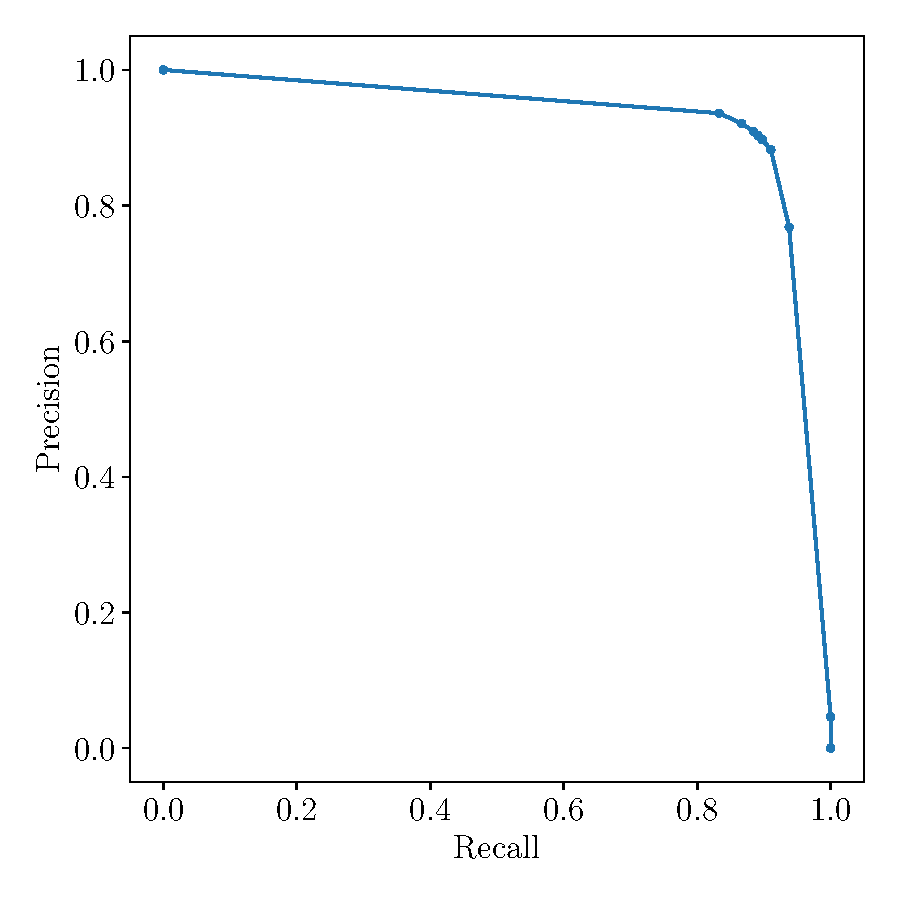
\includegraphics[width=0.6\textwidth]{resources/pdf/precision_recall.pdf}
    \vspace{-1em}
    \caption{Precision-recall curve of our model on the Californian test set.}
    \label{fig:precision_recall}
\end{figure}

As one can see in Figure \ref{fig:precision_recall}, our model performed quite well on the test set, reaching an average precision of \SI{92.51}{\percent}. With a threshold of \num{0.5}, the model detects \SI{89.1}{\percent} of the photovoltaic panels (recall) and what it detects has \SI{90.3}{\percent} of chance to be a photovoltaic panel (precision).

As comparison, to quote DeepSolar's author,

\begin{quote}
    \enquote{DeepSolar achieves a precision of \SI{93.1}{\percent} with a recall of \SI{88.5}{\percent} in residential areas and a precision of \SI{93.7}{\percent} with a recall of \SI{90.5}{\percent} in non-residential areas.}
\end{quote}

We could say that our network performances are quite close to those of DeepSolar, but DeepSolar's test set is quite different from ours, therefore the comparison doesn't make much sense. However, the publishers of the dataset we use also have written a paper \parencite{malof2016deep} about using convolutional neural networks for photovoltaic array detection, where they use the dataset they have published. Quoting them,

\begin{quote}
    \enquote{The CNN is capable of excellent performance, detecting nearly \SI{80}{\percent} of true panels with a precision measure of \SI{72}{\percent}.}
\end{quote}

Our model significantly outperforms these results.

\subsubsection{Fine tuning}

However, when we tried our model on WalOnMap images, it wasn't performing nearly as well, as a lot of shadows\footnote{There are very few building shadows in the Californian images while there are plenty in the Wallonian ones. We believe this is either due to the time of the year where the images were taken or the fact that California is much nearer to the equator than Belgium.} and dark roofs were detected as panels.

Therefore, we \emph{hand-annotated}, using the \enquote{VGG Image Annotator} \parencite{dutta2019vgg}, 661 Wallonian images ($512 \times 512$) in order to \emph{fine tune} our model for a few (20) more epochs. This improved dramatically the performances of the network (cf. Figure \ref{fig:comparison_fine_tuning}) on WalOnMap images.

\begin{figure}[h]
    \centering
    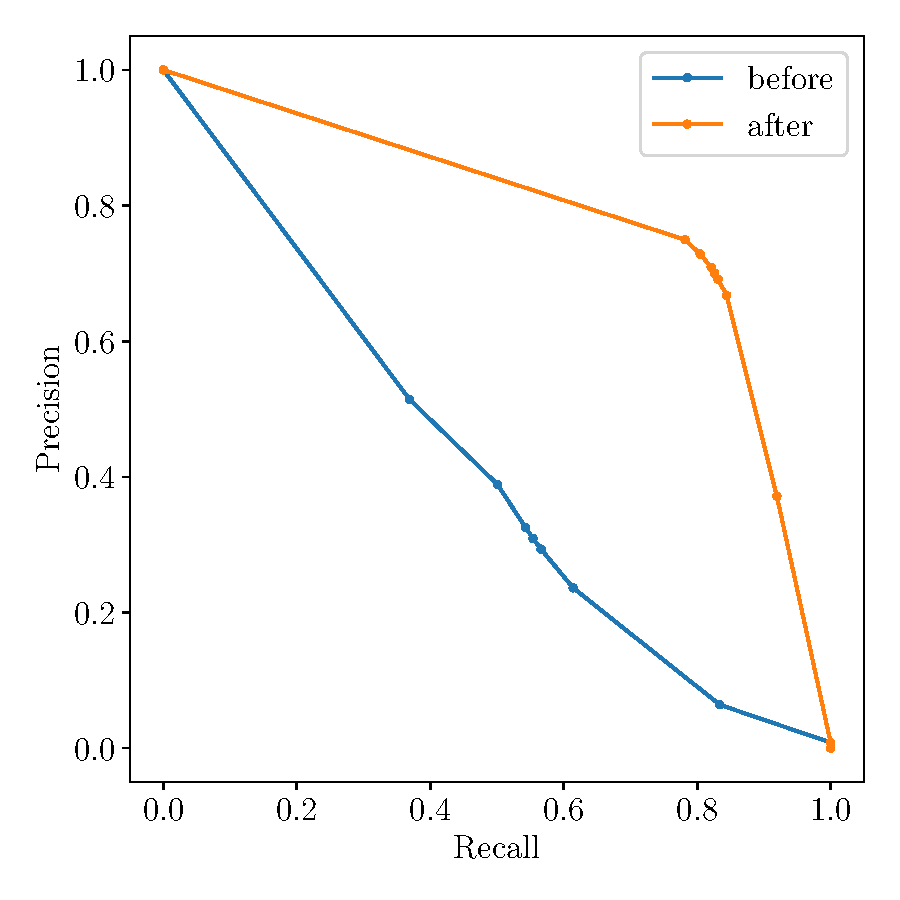
\includegraphics[width=0.6\textwidth]{resources/pdf/before_after.pdf}
    \vspace{-1em}
    \caption{Precision-recall curves of our model on the WalOnMap test set, before and after fine-tuning.}
    \label{fig:comparison_fine_tuning}
\end{figure}

The final average precision reached by our network is \SI{78.3}{\percent}, with \SI{71.3}{\percent} precision and \SI{82.6}{\percent} recall at a threshold of \num{0.5}. Considering we hand-annotated \enquote{only} 661 images, this result is respectable, yet it could certainly profit significantly from a few more images.

\begin{note}
    The WalOnMap test set is composed of 111 of the 661 images we annotated. They were never used for training.
\end{note}

\subsubsection{Province of Liège}

Finally, we applied our fine-tuned model on the \num{846703} tiles of the province of Liège. After about one day and an half of computations\footnote{The computations have been performed using one GTX 1080 Ti GPU of the Alan cluster.}, we obtained the location and shape of \num{65463} photovoltaic installations covering \SI{2554505}{\meter\squared} of surface.

\begin{figure}[h]
    \centering
	\begin{subfigure}{0.31\textwidth}
		\centering
		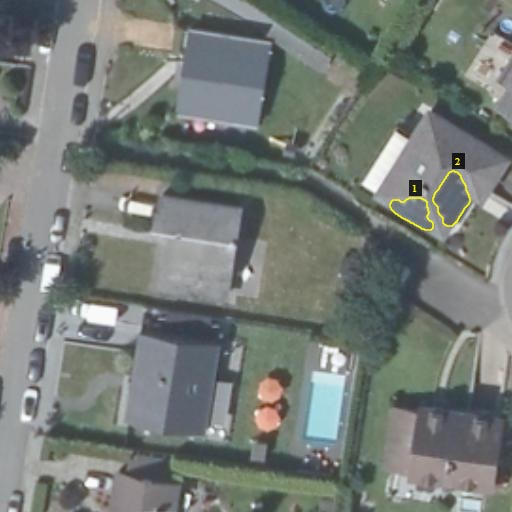
\includegraphics[width=\textwidth]{resources/jpg/609327_533000.jpg}
		\vspace{0em}
	\end{subfigure}
	\hspace{0.5em}
	\begin{subfigure}{0.31\textwidth}
		\centering
		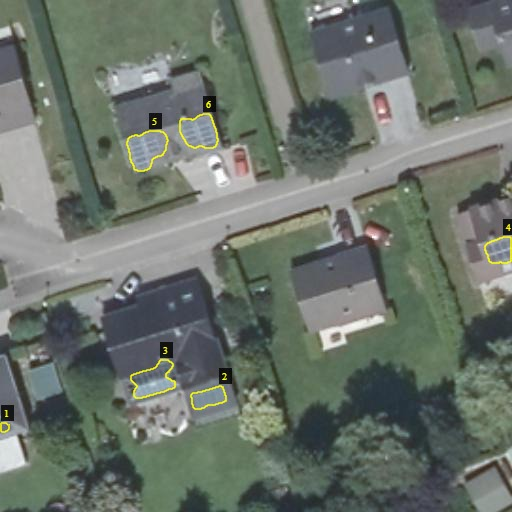
\includegraphics[width=\textwidth]{resources/jpg/609483_533144.jpg}
		\vspace{0em}
	\end{subfigure}
	\hspace{0.5em}
	\begin{subfigure}{0.31\textwidth}
		\centering
		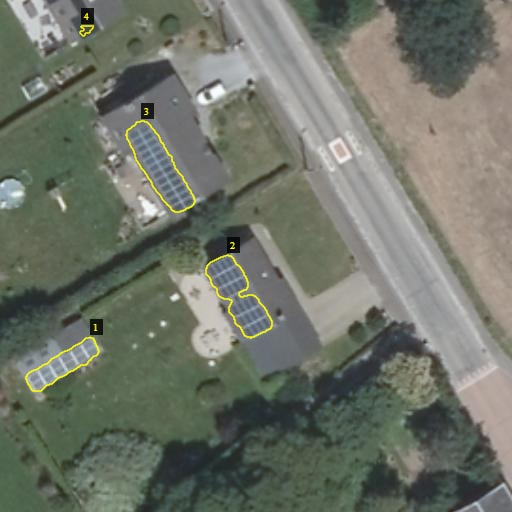
\includegraphics[width=\textwidth]{resources/jpg/609525_533266.jpg}
		\vspace{0em}
	\end{subfigure}
	%%%%%%%%%%%%%%%%%%%%%%%%%%%%%%%%
	\begin{subfigure}{0.31\textwidth}
		\centering
		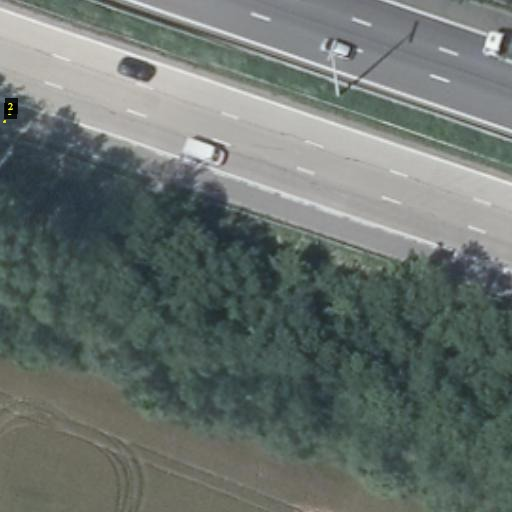
\includegraphics[width=\textwidth]{resources/jpg/609293_532938.jpg}
		\vspace{0em}
	\end{subfigure}
	\hspace{0.5em}
	\begin{subfigure}{0.31\textwidth}
		\centering
		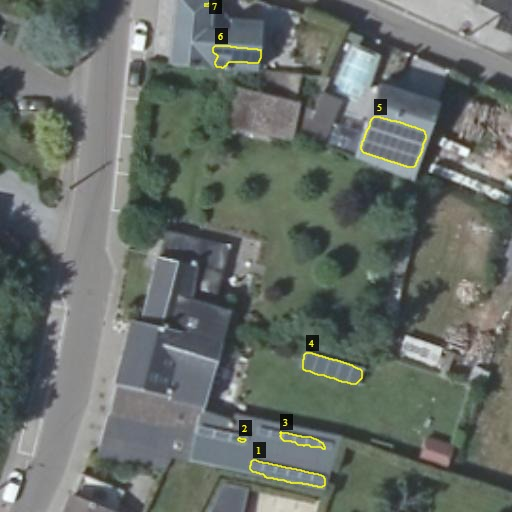
\includegraphics[width=\textwidth]{resources/jpg/609270_533246.jpg}
		\vspace{0em}
	\end{subfigure}
	\hspace{0.5em}
	\begin{subfigure}{0.31\textwidth}
		\centering
		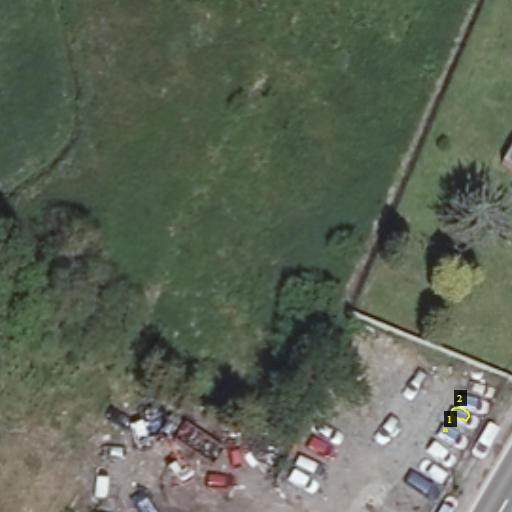
\includegraphics[width=\textwidth]{resources/jpg/609468_532552.jpg}
		\vspace{0em}
	\end{subfigure}
	%%%%%%%%%%%%%%%%%%%%%%%%%%%%%%%%
	\begin{subfigure}{0.31\textwidth}
		\centering
		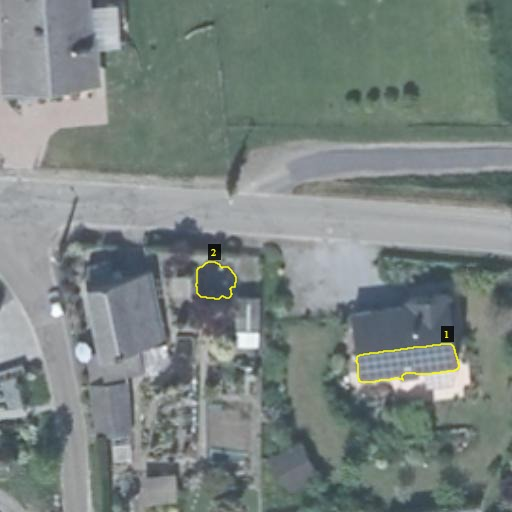
\includegraphics[width=\textwidth]{resources/jpg/609591_532657.jpg}
		\vspace{0em}
	\end{subfigure}
	\hspace{0.5em}
	\begin{subfigure}{0.31\textwidth}
		\centering
		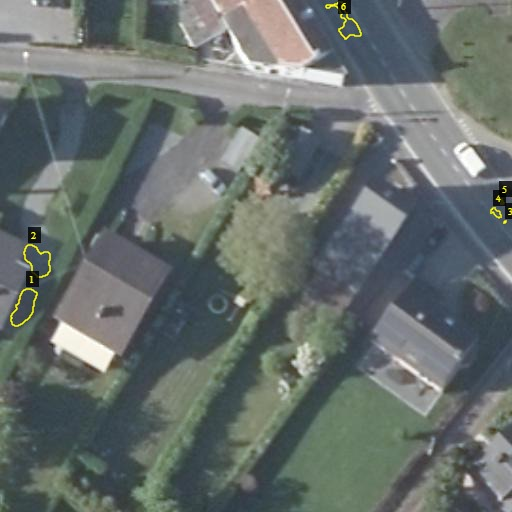
\includegraphics[width=\textwidth]{resources/jpg/609601_533193.jpg}
		\vspace{0em}
	\end{subfigure}
	\hspace{0.5em}
	\begin{subfigure}{0.31\textwidth}
		\centering
		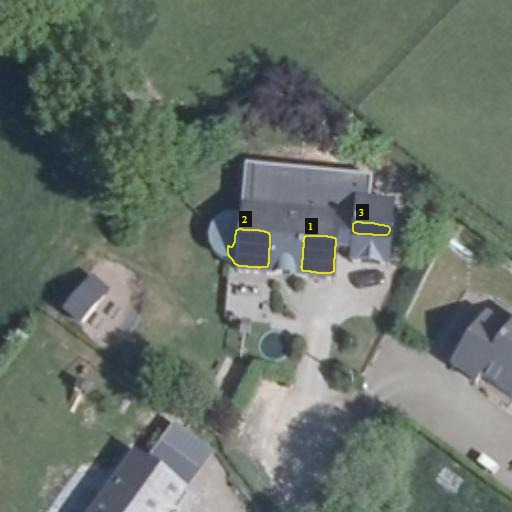
\includegraphics[width=\textwidth]{resources/jpg/609690_533553.jpg}
		\vspace{0em}
	\end{subfigure}
    \caption{Sample of detected photovoltaic panels in the province of Liège.}
\end{figure}

As expected from the previous section results, most panels are accurately detected and segmented, but there are still numerous errors, especially with shadows and canopies (\emph{verrière} in french).

\begin{note}
    As such, the locations and shapes are not usable for the power production model (cf. section \ref{sec:pv_power}). Therefore, we summarized each detected installation into 3 quantities : its geospatial location (latitude and longitude), its surface and an estimate of the surface azimuth angle (cf. section \ref{sec:panelwise}).
\end{note}

\subsection{Limitations and possible improvements}

Although it is still acceptable, the main limitation of our final model is its (average) precision on the WalOnMap images. We don't believe it to be due to the network itself, but rather to the low number of images we hand-annotated. Furthermore, none of the images we annotated were located \emph{in-town}, therefore it is not surprising that most mistakes are made in such areas\footnote{If you wish to see a small (2000) sample of detected panels along with aerial images, you can visit \href{https://www.google.com/maps/d/viewer?mid=1ja5gFenQXNE9TB1rDLuuQsO-H1HH77Jj&usp=sharing}{this website [link]}. However, one should keep in mind that Google's aerial images are much better than those we had access to. Also, the WalOnMap's geospacial localisation is a little translated from the one of Google.}. The most obvious way to improve our results is to annotate much more (varied) images, which we unfortunately had not the time to do.

Another limitation of our model, is that there is no measure of uncertainty about the area of the panels. We tried to use different thresholds in order to compute a kind of variance of the area of each detected installation, but we didn't succeed as, when the threshold changes, some installations merges or aren't detected anymore. This is definitely a sector of possible improvement.

\newpage

\section{Photovoltaic power production}\label{sec:pv_power}

\subsection{Overview of solar power forecasting}

\paragraph{Classification of solar forecasting problems}
There are several time-horizons that can be considered for solar power forecasting tasks:
\begin{itemize}
    \item Very-short-term tasks: forecasts for a few hours ahead;
    \item Short-term tasks: mostly day-ahead forecasts;
    \item Long-term tasks: forecasts for several days.
\end{itemize}
As was explained in the introduction, the goal of this project is to forecast the renewable production for the next day. Hence, we are interested in short-term tasks.

\paragraph{State of the art approaches for day-ahead solar forecasting}
From existing comparisons of photovoltaic forecasting methods \parencite{nespoli2019day} and other case studies \parencite{bocquet2016assessment}, we observed three main standards in solar forecasting:

\begin{enumerate}[label=\arabic*]
    \item \textbf{Statistical methods} These methods are based on sequences of observations measuring different features at successive time instants. They generally only rely on collected data and are not interested in specific features such as panel locations, etc.
    
    Among the mostly used methods, we have regression methods and artificial neural networks. The latter appear to be the most effective ones, allowing to capture and model sharp changes in observed data. Nevertheless, they rely on huge amounts of training data and a well-adapted model architecture, which might be hard to find.
    
    \item \textbf{Physical methods} These methods are mainly based on \emph{Numerical Weather Prediction} (NWP) and rely on panel characteristics in order to make an appropriate prediction. They show some inherent drawbacks: their resolution is quite small (up to maximum \SI{50}{\kilo\meter}) and they achieve better performance when weather conditions are stable, which is certainly not ensured with irradiance data. Hence, they are less robust to sharp changes in observed data.
    
    \item \textbf{Hybrid methods} These methods consist in a combination of the two previous ones, and should solve the issues of one another. Nevertheless, computational complexity increases and the hybrid performance depends on the individual performances of both models, which should be designed for a single plant/location.
\end{enumerate}

\paragraph{Selected approach}
Since we only have access to irradiance measures/forecasts, building a highly complex statistical model around this data seemed to be a pointless task. Furthermore, we were not really interested in reproducing an existing artificial neural network architecture, nor in building one ourselves. Therefore, we moved away from statistical models to opt for physical methods.

As far as physical methods are concerned, we were interested in \emph{physical intuition}; thus, we decided to derive very simple physical models in order to compare them with reference data, and see if such simplified models could actually reach a reasonable level of performance.

Note that we also swiped away hybrid methods since they involve statistical models.

As suggested by the guidelines, we first focused on a smaller scale than Liège, and started looking for a way to model the photovoltaic production at ULiège. The idea was to build a \emph{panelwise} physical model that we would then scale up or simply adapt for the case of Liège, using panels data obtained by processing satellite images in our panel enumerator. By panelwise, we mean that we compute the output power for each panel, or at least for each panel installation. This computation would thus be dependent on the coordinates (latitude and longitude) of each installation, the tilt angle, the area of the installation, ... The results would therefore be inherently dependent on the way and accuracy with which we assess the number of photovoltaic units. Note that, since the ULiège model is only a \emph{sketch model} that we built to check if equation \ref{eq:panelwise_power} gave plausible results, without processing any satellite image, we thought computing its error metrics was not relevant. Hence, we will only display some graphical results where we find it appropriate. 

In a second time, we decided to build a second model, which we named \emph{provincial} model, that computes the photovoltaic production for the whole province of Liège. As will be explained in subsection \ref{subsec:pv_power_data}, moving from the city scale to the province scale was done for the sole reason to have reference production data to fit to.

These two models will be explained in further details in later sections. First, we will introduce the data we managed to collect for this sub-problem.

\subsection{Data collection and processing}
\label{subsec:pv_power_data}

\subsubsection{Photovoltaic production data}
The first step was to gather photovoltaic production data. For our panel-wise model, we needed to get production data from the photovoltaic panels installed at the parking lots of the Sart-Tilman. We obtained access to a live database that provided production data for each minute, which gave us a high-confidence reference for our example model at ULiège.

For production data in Liège, the only publicly available source appeared to be Elia, but it only provided data at a provincial scale. This is the main reason why we considered both photovoltaic models over the whole province of Liège instead of the city of Liège; otherwise we would have had no reference data to compare to. Note that the panelwise model could be applied at any scale, provided that we process the corresponding satellite images. We simply won't have any reference data to compare to.

Elia provides data for each 15-minutes step and gives access to measurements and forecasts, the latter being helpful to compare our model predictions to a reference forecast.

Requesting data to Elia might lead to empty responses or simply missing data for some timestamps. For that reason, we had to treat data carefully to avoid runtime issues in our models. Concerning the photovoltaic production data, we decided to perform a simple interpolation filling for the potential missing data, which seemed quite reasonable.

\subsubsection{Irradiance data}
Finding free of access irradiance data seemed like an impossible task at first. While we collected past irradiance data at the Sart-Tilman (which allowed us to complete and test our first example of panelwise model), the discovery of a data source that could provide both irradiance measures and irradiance forecasts at any location was harder than expected. Considering two independent data sources seemed to be a bad idea due to the likely bias that would exist (adding on top of that the inherent bias present in the forecasts).

Due to the bound on API calls that we would get with any existing free irradiance API, we decided to restrict our data measures to the city of Liège. Obviously, this restriction will impact our production estimates since we aim at predicting at a provincial scale. We decided to opt for Solcast, which offers some credits for academic research purpose and which provides 1000 API calls. As it only allows to request irradiance data for a single production site (for our account type), it perfectly fitted our restriction.

As far as irradiance measures and forecasts are concerned, no complex pre-processing step was needed. 

The first step was to decide for the date and time associated to each measure. Indeed, the API provides measures at a 30-minutes granularity, and each measure consists in an average measure over the past 30 minutes. For instance, the global horizontal irradiance (GHI) reported at 9:00 corresponds to the average GHI measured between 8:30 and 9:00. Hence, we arbitrarily decided to associate to each such measure the date and time corresponding to the middle of the considered averaging period (in the case of our example, it would correspond to 8:45). It also appeared to yield more precise results when doing so rather than when considering the date and time of the end of the period. 

Furthermore, the second step in irradiance pre-processing consisted in building the appropriate data frames in order to store them for caching purposes. Finally, we had to detect potential missing data and perform some action regarding this missing data. To solve this missing data issue, we decided to perform a linear interpolation, as is done for Elia's missing measures.

\subsection{Models description and practical details}
This section will explain in further details the two models described earlier.

\subsubsection{Panelwise model -- \texttt{python/solar\_panelwise.py}} \label{sec:panelwise}
As was already evoked earlier, this model consists in computing the output power for each panel installation. What we plan to do is to use in this model the data (coordinates, area, azimuth) produced by our photovoltaic panels mapping.

After certain research, we derived a formula that estimates the production of a photovoltaic panel depending on several particular angles:
\begin{itemize}
    \item The \textbf{incidence angle} $\theta$ between the sun rays and the normal vector of the panel installation. This angle itself depends on other angles that will be described below.
    \item The \textbf{solar altitude}, $alt$, in order to rescale irradiance measures since what is measured is the horizontal irradiance, not the irradiance that is perpendicular to the panel. It simply corresponds to the angle between the horizontal plane a line drawn from the sun towards the panel.
\end{itemize}

All the following angles intervene in the cosine of the incidence angle $\theta$:
\begin{enumerate}
    \item The \textbf{surface azimuth}: it corresponds to the angle measured between a vertical line going from North to South and the projection on a horizontal plane of the normal to the panel (positive when measured clockwise);
    \item The \textbf{declination angle} $\delta$, which only depends on the day of the year;
    \item The \textbf{latitude} and \textbf{longitude} of the panel;
    \item The \textbf{hour angle} $\omega$, which depends on the location of the panel;
    \item The \textbf{tilt angle} of the panel, $\beta$.
\end{enumerate}
Hence, whenever the cosine of $\theta$ or the sine of $alt$ is negative, it means that the sun is behind the panel or that the sun has set, respectively.

The derived model is the following:
\begin{equation}
    P = \frac{\eta I \cos(\theta) A}{\sin(alt)} \quad [\si{\watt}]
    \label{eq:panelwise_power}
\end{equation}
where $\eta$ is the efficiency of the panel installation, $A$ is the area of the panel and $I$ is the irradiance. For the sake of readability, we decided not to write down the formula of $\cos\theta$. However, it can still be found on this \href{https://www.itacanet.org/the-sun-as-a-source-of-energy/part-3-calculating-solar-angles/}{website} or in the corresponding source code, \texttt{python/solar\_panelwise.py}.

Note that, for the case of ULiège, since we had access to technical specifications of the panel installations, we knew the exact efficiency, tilt, etc. and we also had access to other information such as:
\begin{itemize}
    \item The maximum power bound of the panels
    \item The temperature influence
\end{itemize}
Nevertheless, even if they added a bit of precision, most of these parameters did not play a key role in estimating the output production. Only for the sake of visualization, samples results of the model implemented in equation \ref{eq:panelwise_power} can be observed on Figure \ref{fig:sart_tilman_1} and \ref{fig:sart_tilman_2}. The dates have been chosen according to the available data. 

\begin{figure}[H]
	\centering
	\begin{subfigure}{0.48\textwidth}
		\centering
		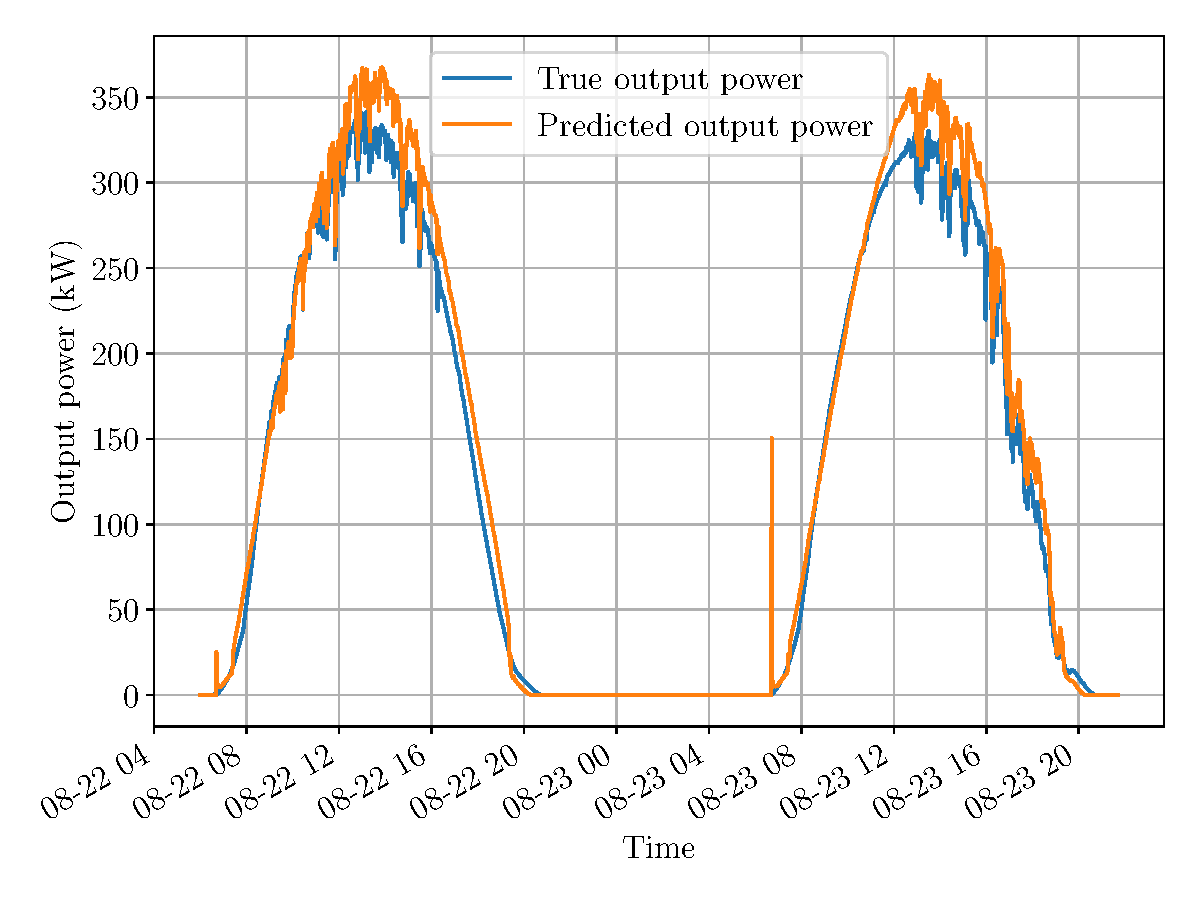
\includegraphics[width=\textwidth]{resources/pdf/sart_tilman (22-08-2019).pdf}
		\vspace{-0.5em}
		\caption{August 22nd and 23rd 2019.}
		\label{fig:sart_tilman_1}
	\end{subfigure}
	\hspace{0.5em}
	\begin{subfigure}{0.48\textwidth}
		\centering
		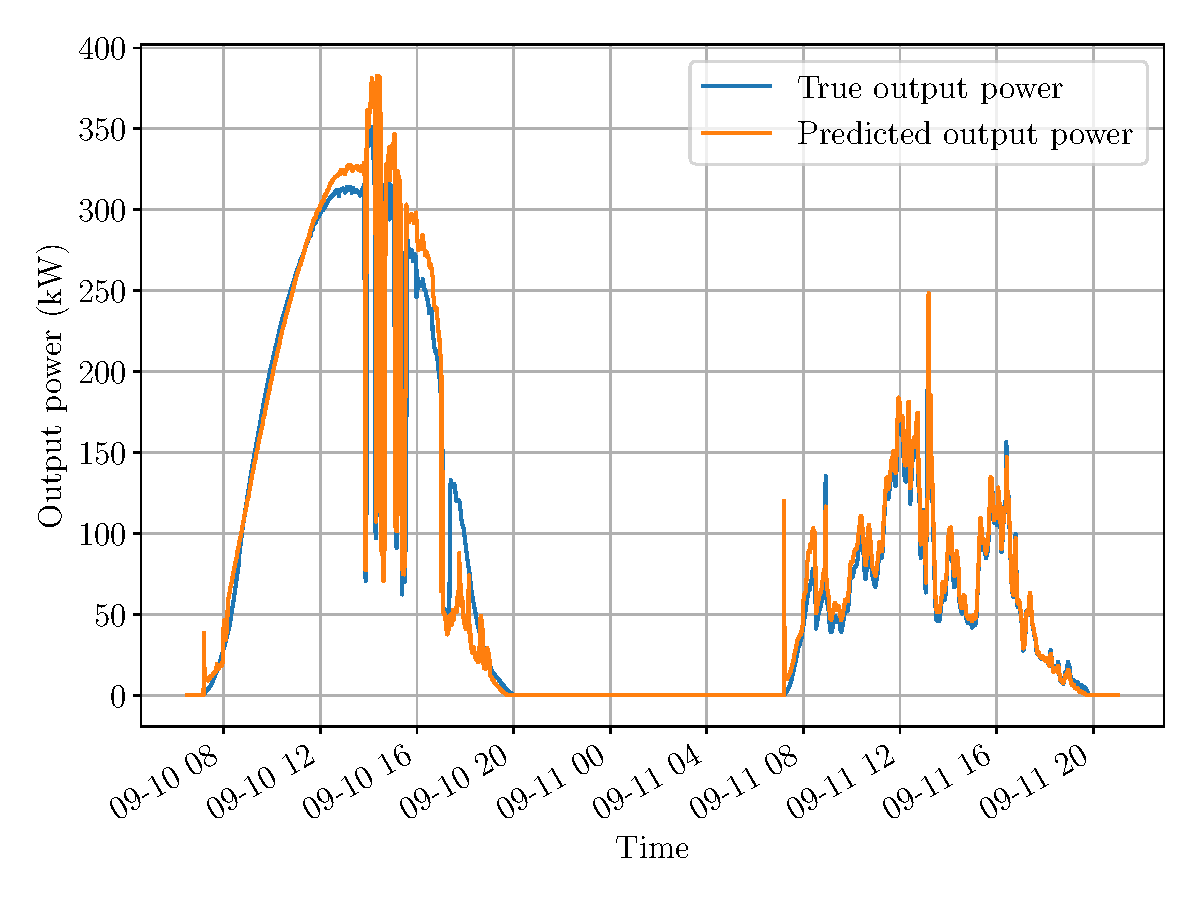
\includegraphics[width=\textwidth]{resources/pdf/sart_tilman (10-09-2019).pdf}
		\vspace{-0.5em}
		\caption{September 10th and 11th 2019.}
		\label{fig:sart_tilman_2}
	\end{subfigure}
	\caption{Samples of the physical model derived in equation \ref{eq:panelwise_power}, for ULiège.}
	\label{fig:sart_tilman}
\end{figure}
Note that the presence of peaks is due to the fact that both the cosine of the incidence angle and the sine of the altitude are very small (but positive) at these time steps. This seems to happen because of the small time granularity we used for ULiège (1 minute).

From this model, we can thus get an estimate of the output power of photovoltaic panels at any scale, provided that we have access to specific information about them, namely the latitude, longitude, area and surface azimuth.

Taking uncertainties into account for parameters such as $\eta$ and $\beta$ was only slightly performed for this model, for several reasons. Firstly, modeling uncertainties for $\beta$ seemed to be a hard task since it is entangled in $\cos\theta$ and thus we couldn't directly interact with it through a PyStan\footnote{PyStan is a Python probabilistic framework, which is particularly useful to model uncertainties about parameters in physical models, when it comes to making inference using these parameters.} model. 

Hence, the only remaining parameter we could toy with was $\eta$, which was not completely sufficient to model correct and reasonable uncertainties.  However, we still managed to model some uncertainty about $\eta$, making the panelwise model less rigid, yet not perfect.

\begin{note}
    All the following equations are expressed in \si{\mega\watt}.
\end{note}
Modeling uncertainty about $\eta$ was done using as prior a normal distribution centered around the predefined value for $\eta$ (which we set equal to the efficiency of the panels at ULiège, i.e. $0.162$), with a scale of \num{0.1}:
\begin{equation*}
    \eta \simeq \mathcal{N}(0.162, \num{e-2})
\end{equation*}
To fit the posterior distribution of this parameter, we used Elia's production measurements over the last 7 days and modeled these measurements as a normal distribution centered around $\eta$ times $naive\_power$ :
\begin{equation*}
    true\_power \simeq \mathcal{N}(\eta \times naive\_power, 100^2)
\end{equation*}
where $$naive\_power = \frac{I \cos(\theta) A}{\sin(alt)}$$

The large scale seemed to increase convergence speed.

Finally, we obtain the predicted production power using the posterior distribution on $\eta$ as well as by modeling a new quantity, \emph{forecast\_power}, which corresponds in some sense to the true forecasted power. This true forecasted power is obviously unknown, and we model it as the mean of a normal distribution from which the $naive\_power$ computed using irradiance forecasts is sampled:
\begin{equation*}
    naive\_forecast\_power \simeq \mathcal{N}(forecast\_power, 10^2)
\end{equation*}
Then, we compute the predicted production by modeling it as a normal distribution centered around $\eta$ times $forecast\_power$, where both factors are sampled from their posterior distributions :
\begin{equation*}
    predicted\_power \simeq \mathcal{N}(\eta \times forecast\_power, 10^2)
\end{equation*}
Nevertheless, one should keep in mind that the main contribution to this model will correspond, in the end, to the total estimated area of photovoltaic units, which will be mainly responsible for the computed output power. The uncertainty should thus rather come from this area than from panels hyperparameters.

Note that we also tried to model these uncertainties in a different way, considering each panel installation's output power (computed in \ref{eq:panelwise_power}) as being weighted by some unknown, which would represent our uncertainty, and fitting these weights with PyStan with respect to Elia's production measurements. Unfortunately, the corresponding model became extremely slow and we decided to drop that idea.

\subsubsection{Provincial model -- \texttt{python/solar\_provincial.py}}
In this second model, we wish to estimate the photovoltaic production at the provincial scale, without having detailed information about the locations of the panels, their areas, etc. 

However, we found a data file containing detailed information, among others about the installed power (in \si{\kilo\voltampere}, which can be assimilated to \si{\kilo\watt}, for simplifications) of photovoltaic panels for each municipality in the province of Liège. From there, we could get a first estimate of the installed power for the whole province.

To get an estimate of the power production, we need to compute a quantity expressed in Watts. Since we have the installed power (\si{\kilo\watt Peak}) and the irradiance (\si{\watt/\meter\squared}), we need another quantity that would, in some sense, \emph{cancel} the installed power to get something in \si{\meter\squared} in the end. For that purpose, we defined a parameter $peak\_area$, corresponding to the average surface of panels per \si{\kilo\watt Peak} (\si{\meter\squared/\kilo\watt Peak}). Hence, multiplying the installed power by this parameter gives us the quantity we are looking for: the area of photovoltaic panels installed in the province of Liège.

From there, the provincial model is quite straightforward:
\begin{equation}
    P = \eta I A \quad [\si{\watt}]
\end{equation}
where $\eta$ is the panel efficiency, $I$ is the irradiance and $A = peak\_area \times \si{\kilo\voltampere}$ is the area of panels in the province (with \si{\kilo\voltampere} being the installed power).

Exactly like for the previous model, all parameters are arbitrarily fixed and the model is thus very rigid and will very likely perform well only by chance. To solve this issue, we decided to implement a PyStan program that would be in charge of modeling appropriate uncertainties for all factors of the equation. 

In this program, we model the uncertainties with very simple equations and distributions, in the following manner\footnote{For a more code-like representation, please refer to \texttt{python/solar\_provincial.py}}. We will compute the posterior of 4 quantities, using Elia's measurements (modeled as a normal distribution centered around the product of these 4 quantities). 
\begin{note}
    The order of magnitude of the units used in this model are \si{\kilo\watt}, not \si{\watt} nor \si{\mega\watt}.
\end{note}
\begin{enumerate}
    \item The prior of the efficiency $\eta$ is modeled using a normal distribution, centered around the value we arbitrarily fixed (ETA) and with a scale of 0.01.
    \begin{equation*}
        \eta \simeq \mathcal{N}(\text{ETA}, 0.01)
    \end{equation*}
    \item The prior of the peak area is modeled using a normal distribution too, centered around the predefined value (PEAK\_AREA) and with a scale of 1 \si{\meter\squared/\kilo\watt Peak}.
    \begin{equation*}
        peak\_area \simeq \mathcal{N}(\text{PEAK\_AREA}, 1)
    \end{equation*}
    \item The observed irradiance measures are also assumed to be uncertain. Hence, we modeled a new quantity ($I$) representing the true observed irradiance, as the mean of a normal distribution where the API measures ($I\_obs$) are sampled from, with a scale of \SI{1}{\watt}. The uncertainty will thus be quite small for the irradiance but this is for the sake of coherence with respect to the real world. Indeed, when setting a higher scale, the mean distribution of the irradiance was always strictly positive, which made no sense for night observations. Nevertheless, this behavior still slightly remains, yet it can be considered as negligible.
    \begin{equation*}
        I\_obs \simeq \mathcal{N}(I, 0.001^2)
    \end{equation*}
    \item The installed power's prior is modeled as a uniform distribution. Therefore, the uncertainty will be initially higher for that parameter, which is something we wish: as it represents the installed power for the whole province, we want to allow this parameter to vary as much as possible in order to fit well Elia's measurements.
\end{enumerate}
As was said above, we will build their posterior distributions thanks to the following distribution, where $true\_power$ corresponds to Elia's production measurements (expressed in \si{\kilo\watt}):
\begin{equation*}
    true\_power \simeq \mathcal{N}(\eta \times I \times peak\_area \times \si{\kilo\voltampere}, (10^5)^2)
\end{equation*}
Building the posterior predictive model is done in a similar way. Indeed, the forecast irradiance is modeled in the same manner as the observed irradiance, and we simply model the predicted output power as a normal distribution centered around the product of the 4 previous quantities, replacing $I$ by $I\_for$, the quantity representing the true irradiance forecasts. We thus have:
\begin{equation*}
    predicted\_power \simeq \mathcal{N}(\eta \times I\_for \times peak\_area \times \si{\kilo\voltampere}, 100^2)
\end{equation*}
From this predicted power, we can retrieve the mean distribution and compare this mean distribution with Elia's measurements (if they are available, which won't be the case in a real-world setting) or with Elia's forecasts.

\subsection{Analysis of the models accuracy}
In order to assess the quality of both models, we applied the following procedure. For both models, we fit and construct the posterior models using Elia's measurements over the past 7 days, then we predict for the current day using the predictive model defined in the previous section. For instance, if we wish to predict the power production for April 15th, we build our posterior model using measurements from April 8th up to April 14th and predict using the forecasts requested for April 15th.

In order to get representative results, we firstly conducted this procedure for the whole year of 2019, i.e. we predicted for each day of 2019. However, since we had no access to past irradiance forecasts, we had to perform these tests using irradiance measures only. Doing so will necessarily bias the results in an optimistic way since irradiance measures will always be more accurate than irradiance forecasts. This can be observed on Figure \ref{fig:comparison_meas_meas_meas_for_panelwise} and \ref{fig:comparison_meas_meas_meas_for_provincial}, where we compared the use of irradiance measures and irradiance forecasts for our predictions.

We chose to compute 2 specific metrics, namely the mean-square error (MSE) and the root mean-square error (RMSE), for each day. The RMSE, in some sense, will give us a measure of the error that we will make for the predicted day. Note that these metrics are computed after removing night observations: that is, we only consider points at time steps where Elia's production measurements are non zero. Then, we simply compute the average metrics along with their standard deviation.

As baseline models, we constructed 2 very simple models:
\begin{enumerate}
    \item The first one consists in predicting as produced power for day $D$ the power measured by Elia for day $D-1$.
    \item The second one consists in predicting as produced power for day $D$ the average power measured by Elia over the past 7 days.
\end{enumerate}

Along with those, we also assessed the forecasts made by Elia as well as our naive predictive model (which uses fixed parameters, hence being more rigid). Note that, for our posterior model, we compute the metrics with respect to the mean distribution of the posterior model.

A general remark to note for our two posterior models is that the quality of their predictions will mainly depend on the training period, i.e. on the past 7 days of measurements. Hence, if the training period is not very representative of the power that will be produced on the predicting day, it is very likely that our parameters will wrongly fit the training period and thus yield poor results for the predicting day. This could potentially be solved by training on a much larger period, although we did not really try doing so.  We tested increasing arbitrarily to 3 months of training data but it yielded very poor performance as far as time complexity is concerned. Furthermore, fitting on the past 7 days seemed intuitively to be a reasonable assumption to represent how the irradiance would evolve through time.

These results can be found in Table \ref{tab:results_2019}. From these, we can see that some are very accurate and perform better or equivalently to the baselines, while some others perform very poorly. For most cases, Elia's production forecasts are very close to the measured production curve. This could be explained by the fact that Elia probably does not rely on such a simple model to compute its forecasts. The simplicity of our models is clearly a limitation, even though we are still satisfied with the results produced, on average. Furthermore, the irradiance curve seems to mainly control our predictions, as will be discussed in Section \ref{subsec:limitations_solar}.

We can observe from Table \ref{tab:results_2019} that both posterior predictive models perform similarly. However, the prior models show completely different performances. Indeed, the prior panelwise model has a much higher MSE on average. This could be due to the accuracy of our photovoltaic panels mapping, which seems to slightly overestimate the total area of detected panels (as can be seen on Figure \ref{fig:good_results_april_5th} and \ref{fig:bad_results_april_3rd}). Hence, since we use a fixed efficiency $\eta$, this efficiency seems to be too high most of the time, and too low for some other cases.

\begin{table}[H]
\centering
\begin{tabular}{l|l|l}
                           & MSE     & RMSE
                           \\ \hline
Prior panelwise model      & 2852.73 & 49.25 $\pm$ 20.68
\\\hline
Posterior panelwise model  & 510.84  & 20.06 $\pm$ 10.42 \\ \hline
Prior provincial model     & 608.98  & 21.94 $\pm$ 11.31 \\ \hline
Posterior provincial model & 431.23  & 18.49 $\pm$ 9.46  \\ \hline
Baseline 1                 & 2195.60 & 38.87 $\pm$ 26.19 \\ \hline
Baseline 2                 & 1816.74 & 37.34 $\pm$ 20.56 \\ \hline
Elia's forecast            & 381.85  & 16.79 $\pm$ 10.01
\end{tabular}
\caption{Mean MSE and mean RMSE, along with standard deviation, for 2019 (using irradiance measurements), in \si{\mega\watt}.}
\label{tab:results_2019}
\end{table}


\begin{table}[]
\centering
\begin{tabular}{l|l|l}
                           & MSE     & RMSE              \\ \hline
Prior panelwise model      & 5316.57 & 62.85 $\pm$ 37.66 \\ \hline
Posterior panelwise model  & 1563.30 & 32.23 $\pm$ 23.33 \\ \hline
Prior provincial model     & 2210.83 & 42.44 $\pm$ 20.62 \\ \hline
Posterior provincial model & 1595.59 & 32.63 $\pm$ 23.48 \\ \hline
Baseline 1                 & 2616.99 & 36.34 $\pm$ 36.68 \\ \hline
Baseline 2                 & 2339.52 & 40.87 $\pm$ 26.34 \\ \hline
Elia's forecast            & 324.85  & 15.16 $\pm$ 10.11
\end{tabular}
\caption{Mean MSE and mean RMSE along with standard deviation, for April 2020 (using irradiance forecasts), in \si{\mega\watt}.}
\label{tab:results_april}
\end{table}

\begin{figure}[H]
	\centering
	\begin{subfigure}{0.48\textwidth}
		\centering
		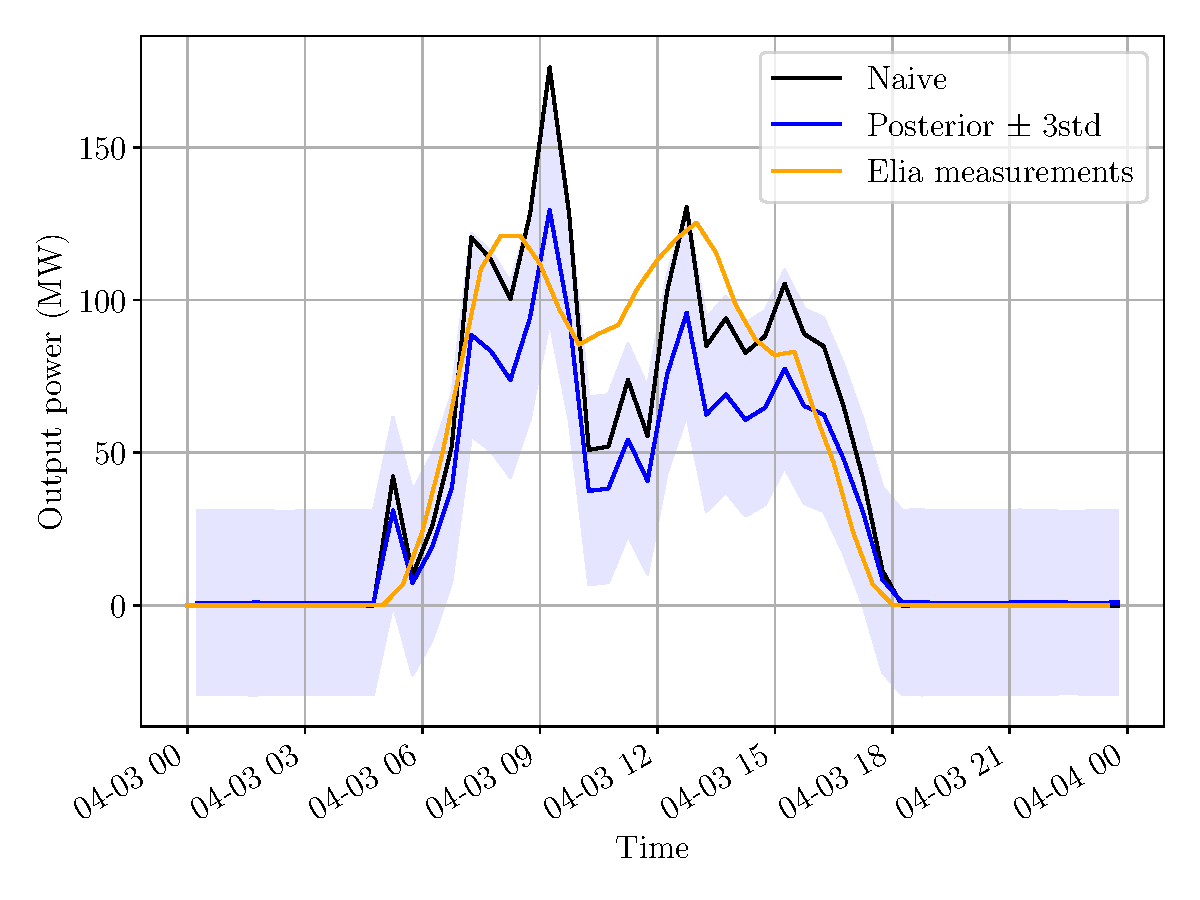
\includegraphics[width=\textwidth]{resources/pdf/solar_panelwise_meas_meas (START_FOR 03-04-2020).pdf}
		\caption{Panelwise model predicting with irradiance measurements.}
		\label{fig:panelwise_meas_meas}
	\end{subfigure}
	\hspace{0.5em}
	\begin{subfigure}{0.48\textwidth}
		\centering
		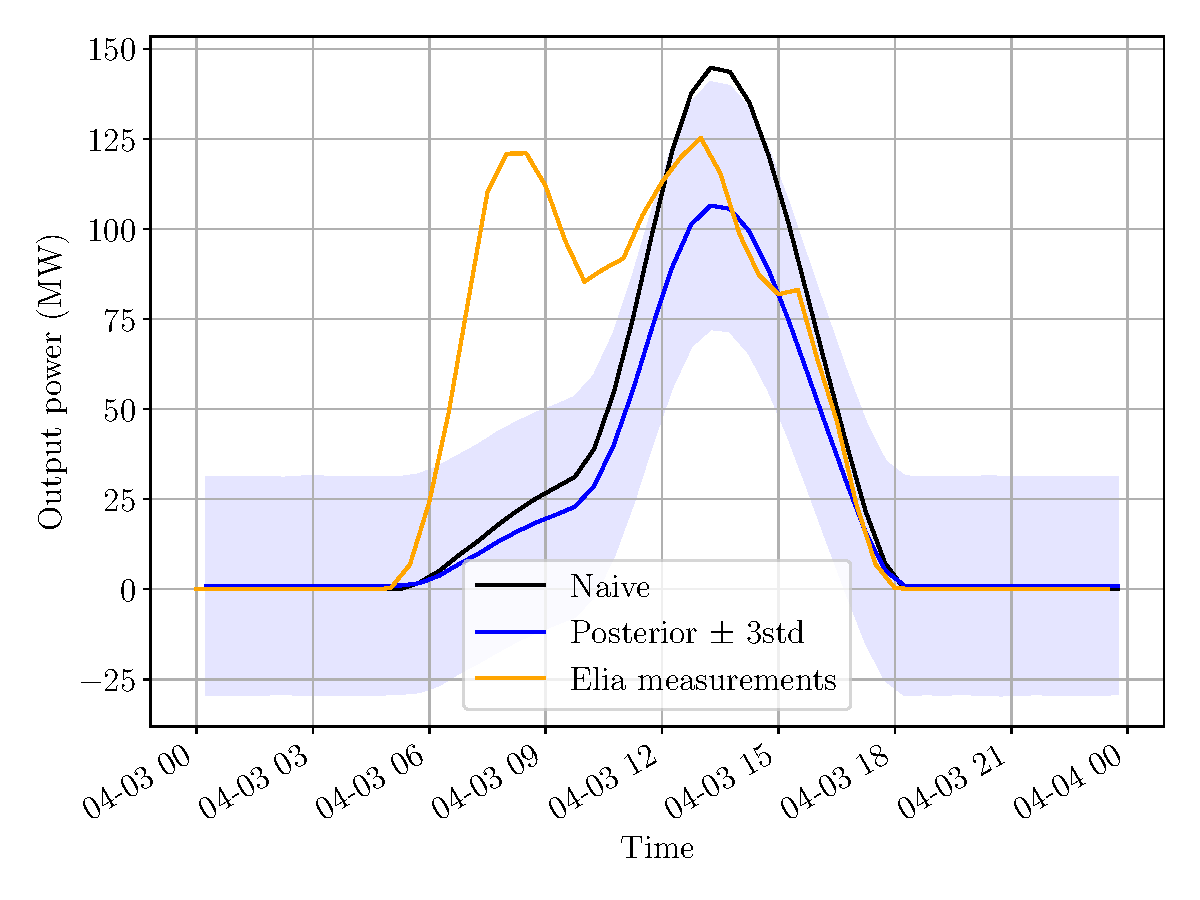
\includegraphics[width=\textwidth]{resources/pdf/solar_panelwise_meas_for (START_FOR 03-04-2020).pdf}
		\caption{Panelwise model predicting with irradiance forecasts.}
		\label{fig:panelwise_meas_for}
	\end{subfigure}
	\caption{Comparison of panelwise model with irradiance measurements/forecasts (April 3rd 2020).}
	\label{fig:comparison_meas_meas_meas_for_panelwise}
\end{figure}

\begin{figure}[H]
	\centering
	\begin{subfigure}{0.48\textwidth}
		\centering
		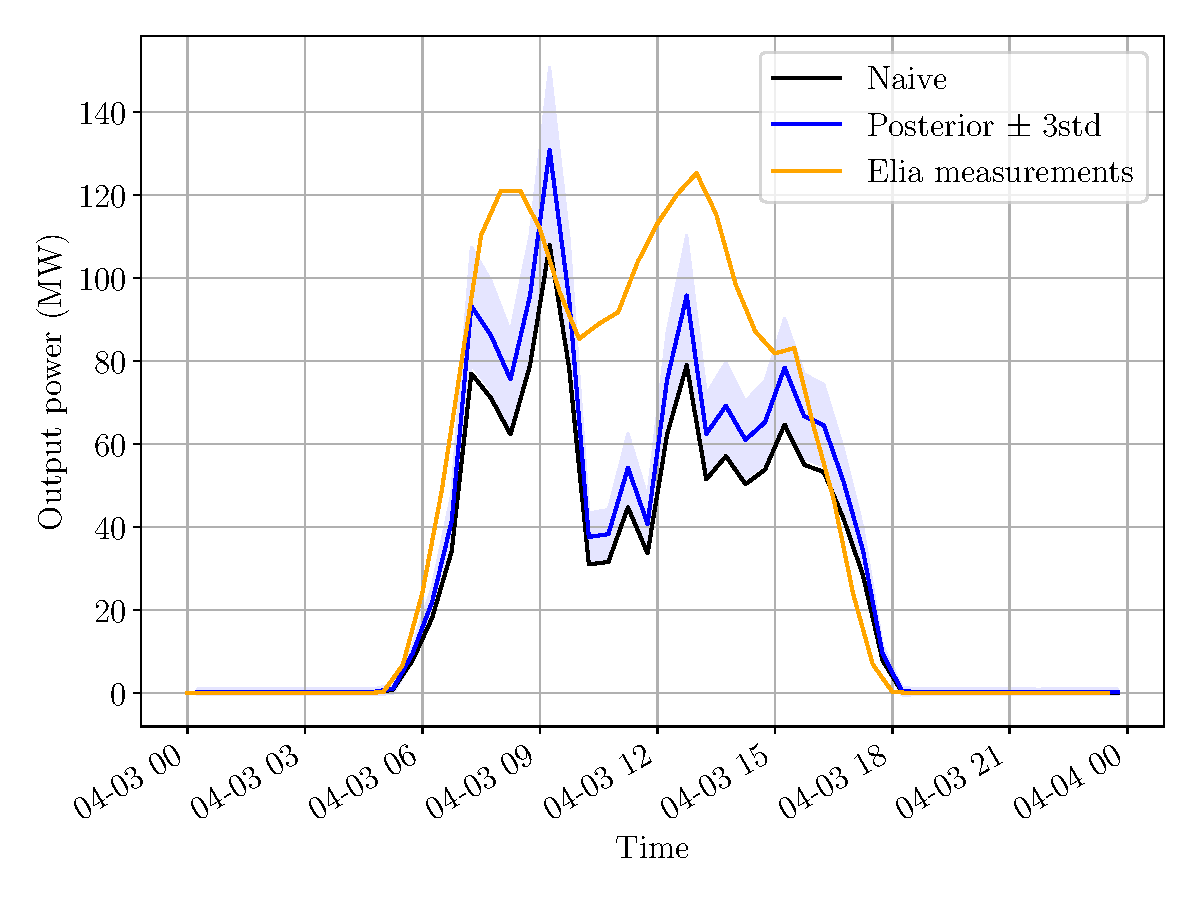
\includegraphics[width=\textwidth]{resources/pdf/solar_provincial_meas_meas (START_FOR 03-04-2020).pdf}
		\caption{Provincial model predicting with irradiance measurements.}
		\label{fig:panelwise_meas_meas}
	\end{subfigure}
	\hspace{0.5em}
	\begin{subfigure}{0.48\textwidth}
		\centering
		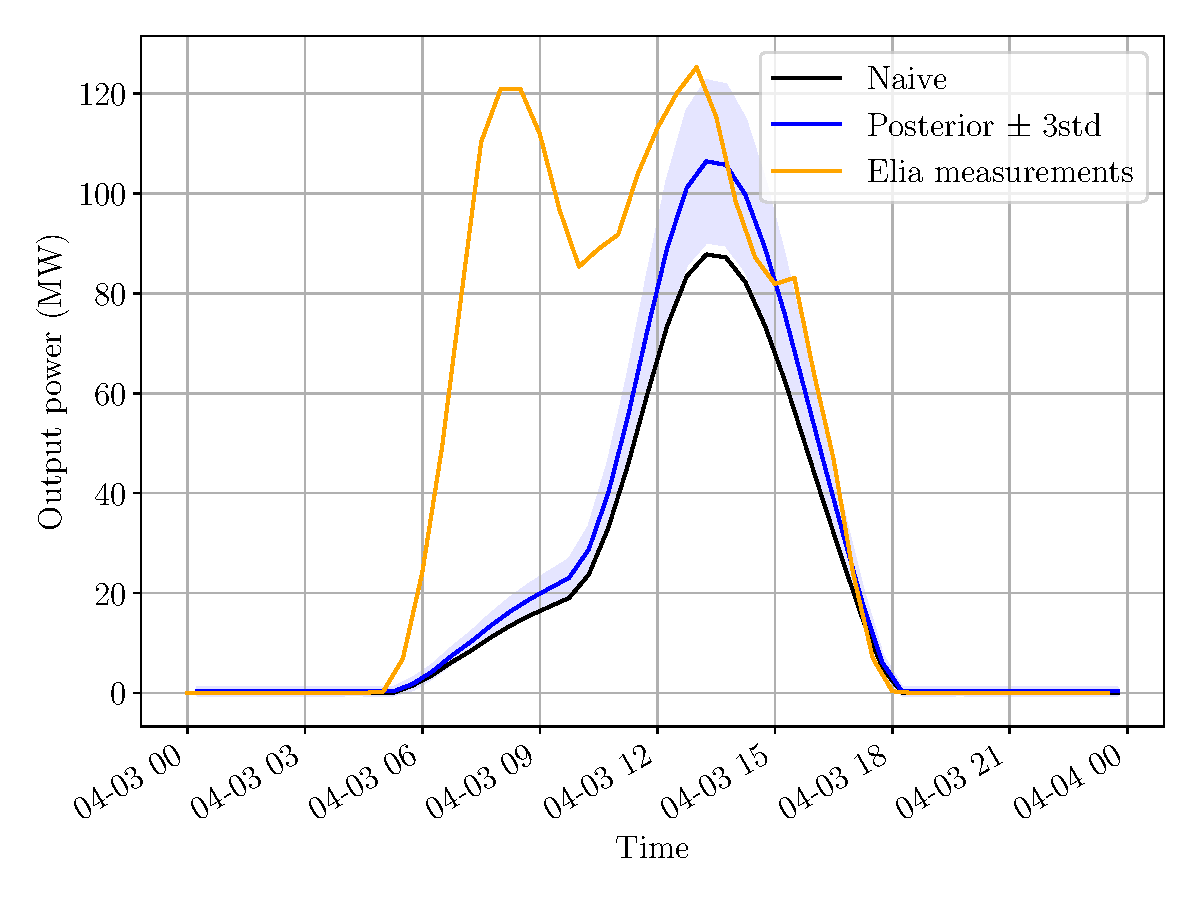
\includegraphics[width=\textwidth]{resources/pdf/solar_provincial_meas_for (START_FOR 03-04-2020).pdf}
		\caption{Provincial model predicting with irradiance forecasts.}
		\label{fig:panelwise_meas_for}
	\end{subfigure}
	\caption{Comparison of provincial model with irradiance measurements/forecasts (April 3rd 2020).}
	\label{fig:comparison_meas_meas_meas_for_provincial}
\end{figure}

To get representative results using irradiance forecasts instead of irradiances measurements, we conducted the same testing procedure for the whole month of April. Consequently, the results (in Table \ref{tab:results_april}) appeared to be worse than those obtained for 2019, as could be expected. Some sample executions can be observed on Figure \ref{fig:good_results_april_4th}, \ref{fig:good_results_april_5th}, \ref{fig:bad_results_april_3rd} and \ref{fig:bad_results_april_7th}. Once again, we can see that Elia outperforms all models, and that both posterior models perform similarly. However, as could be noticed in Table \ref{tab:results_2019}, the prior panelwise model performs much worse than the prior provincial model.

Nevertheless, we can see that in both cases (using irradiance measurements and irradiance forecasts), both posterior models seem to perform better than our baseline models. The performance of the latter will totally depend on the measured production in the past. Hence, if that past production is not representative at all of the future production, results will be bad. Overall, the \emph{averaging} baseline model should be a little bit more robust than the one that simply reproduces the production of the previous day, unless production measurements are very similar for several consecutive days.

\begin{figure}[H]
	\centering
	\begin{subfigure}{0.48\textwidth}
		\centering
		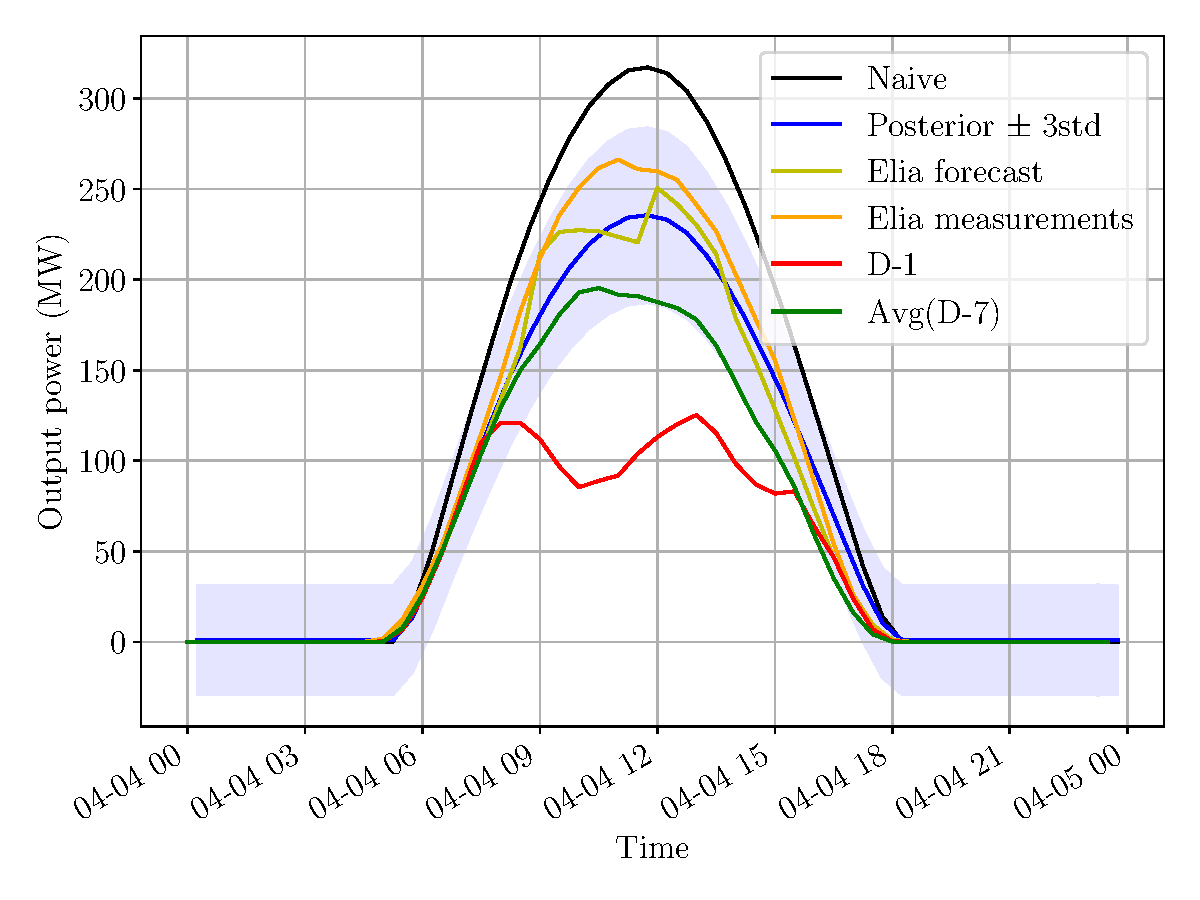
\includegraphics[width=\textwidth]{resources/pdf/solar_panelwise (START_FOR 04-04-2020).pdf}
		\caption{Panelwise model (using irradiance forecasts).}
		\label{fig:panelwise_good_1}
	\end{subfigure}
	\hspace{0.5em}
	\begin{subfigure}{0.48\textwidth}
		\centering
		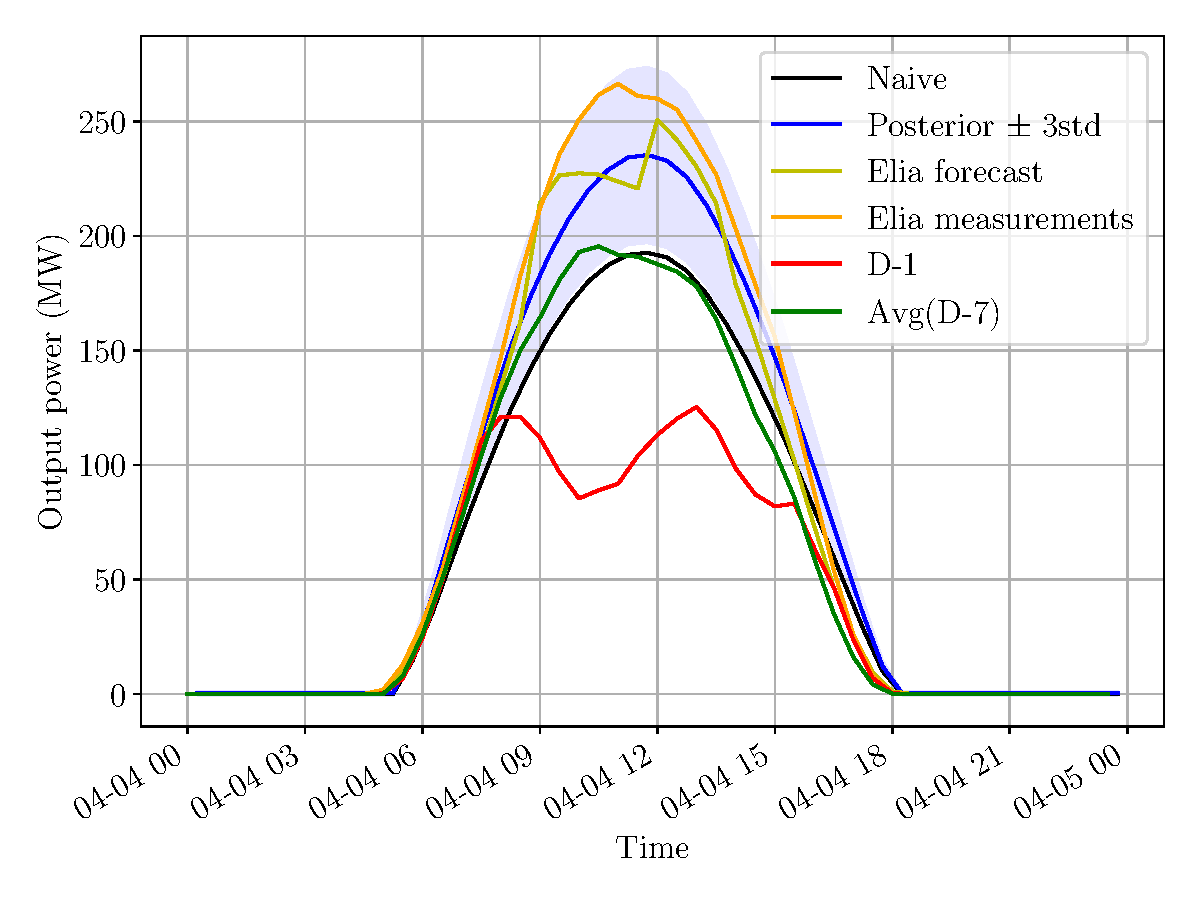
\includegraphics[width=\textwidth]{resources/pdf/solar_provincial (START_FOR 04-04-2020).pdf}
		\caption{Provincial model (using irradiance forecasts).}
		\label{fig:provincial_good_1}
	\end{subfigure}
	\caption{Samples of accurate results with both models (April 4th 2020) and the baselines.}
	\label{fig:good_results_april_4th}
\end{figure}

\begin{figure}[H]
	\centering
	\begin{subfigure}{0.48\textwidth}
		\centering
		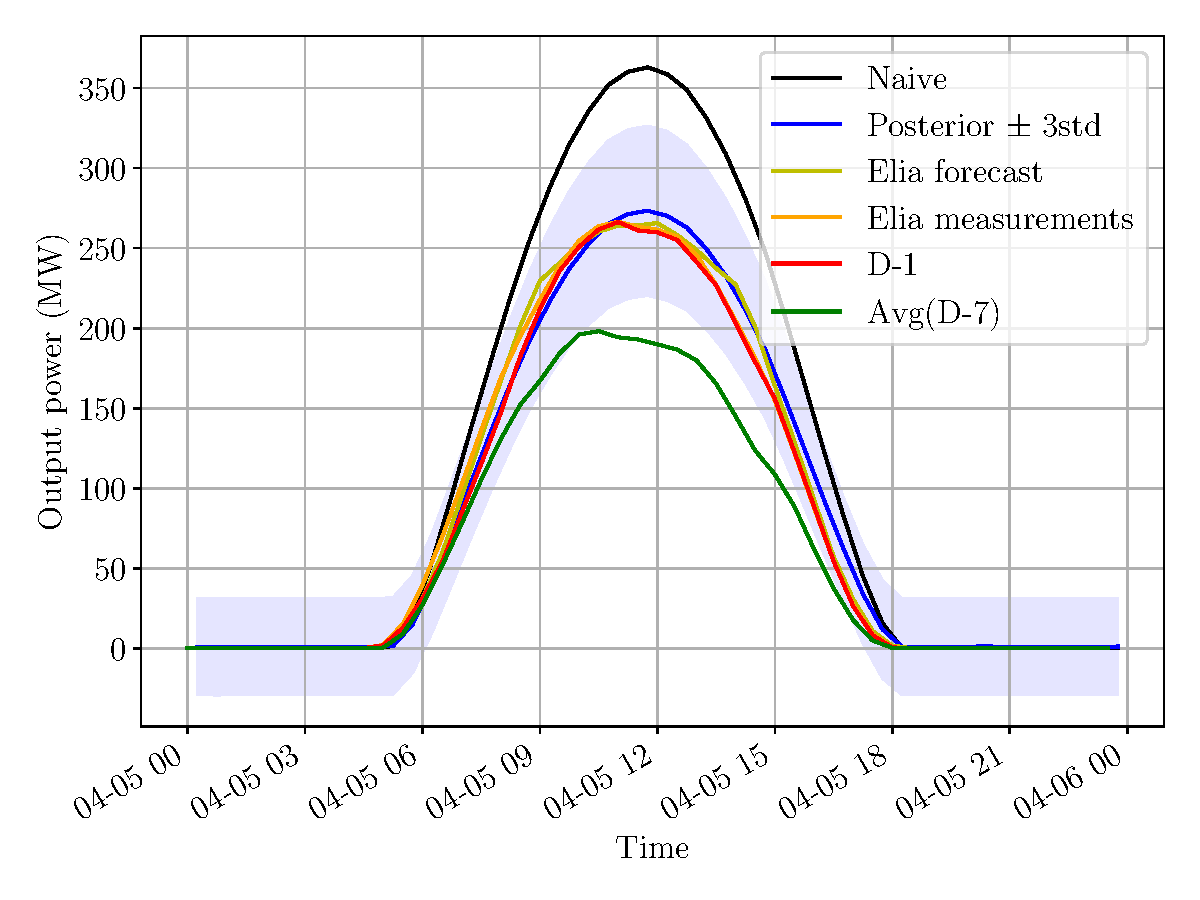
\includegraphics[width=\textwidth]{resources/pdf/solar_panelwise (START_FOR 05-04-2020).pdf}
		\caption{Panelwise model (using irradiance forecasts).}
		\label{fig:panelwise_good_2}
	\end{subfigure}
	\hspace{0.5em}
	\begin{subfigure}{0.48\textwidth}
		\centering
		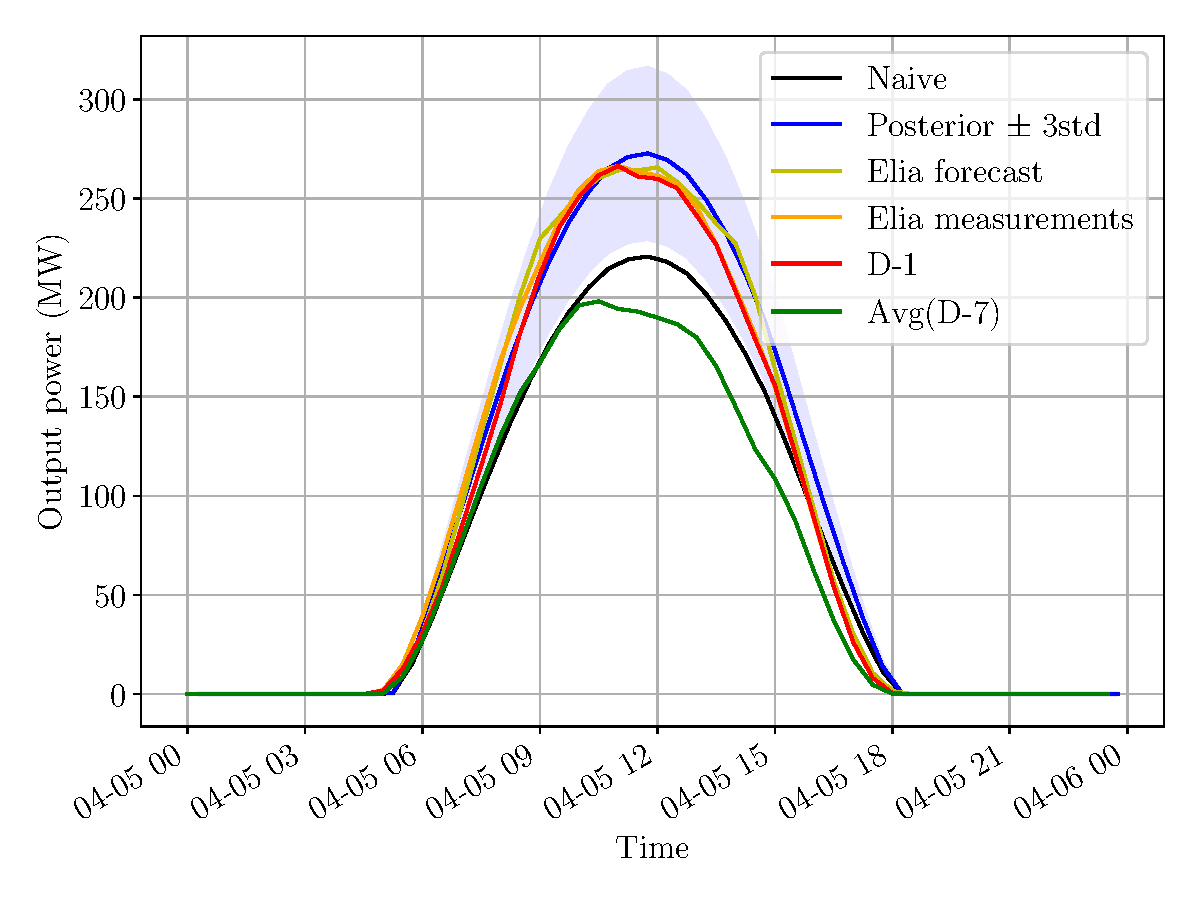
\includegraphics[width=\textwidth]{resources/pdf/solar_provincial (START_FOR 05-04-2020).pdf}
		\caption{Provincial model (using irradiance forecasts).}
		\label{fig:provincial_good_2}
	\end{subfigure}
	\caption{Samples of accurate results with both models (April 5th 2020) and the baselines.}
	\label{fig:good_results_april_5th}
\end{figure}

\begin{figure}[H]
	\centering
	\begin{subfigure}{0.48\textwidth}
		\centering
		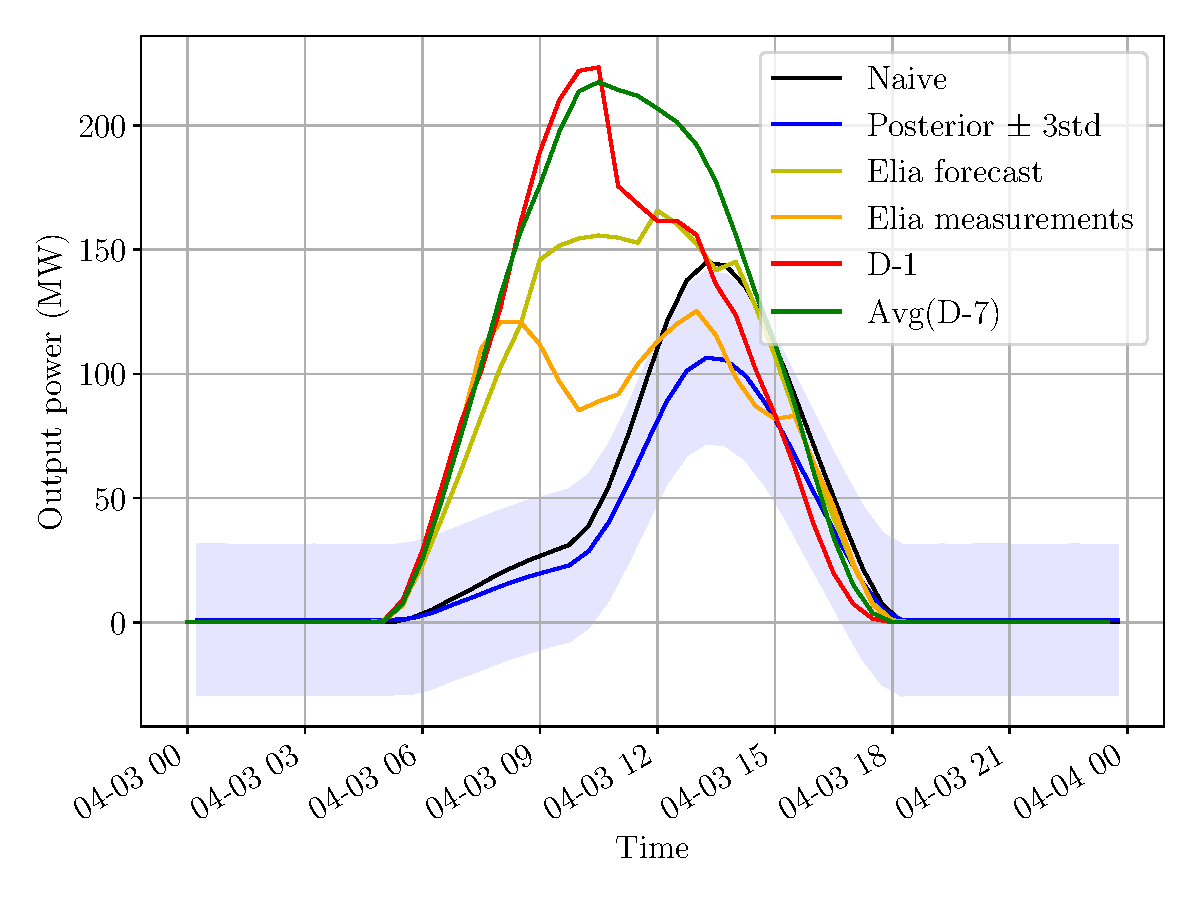
\includegraphics[width=\textwidth]{resources/pdf/solar_panelwise (START_FOR 03-04-2020).pdf}
		\caption{Panelwise model (using irradiance forecasts).}
		\label{fig:panelwise_bad_1}
	\end{subfigure}
	\hspace{0.5em}
	\begin{subfigure}{0.48\textwidth}
		\centering
		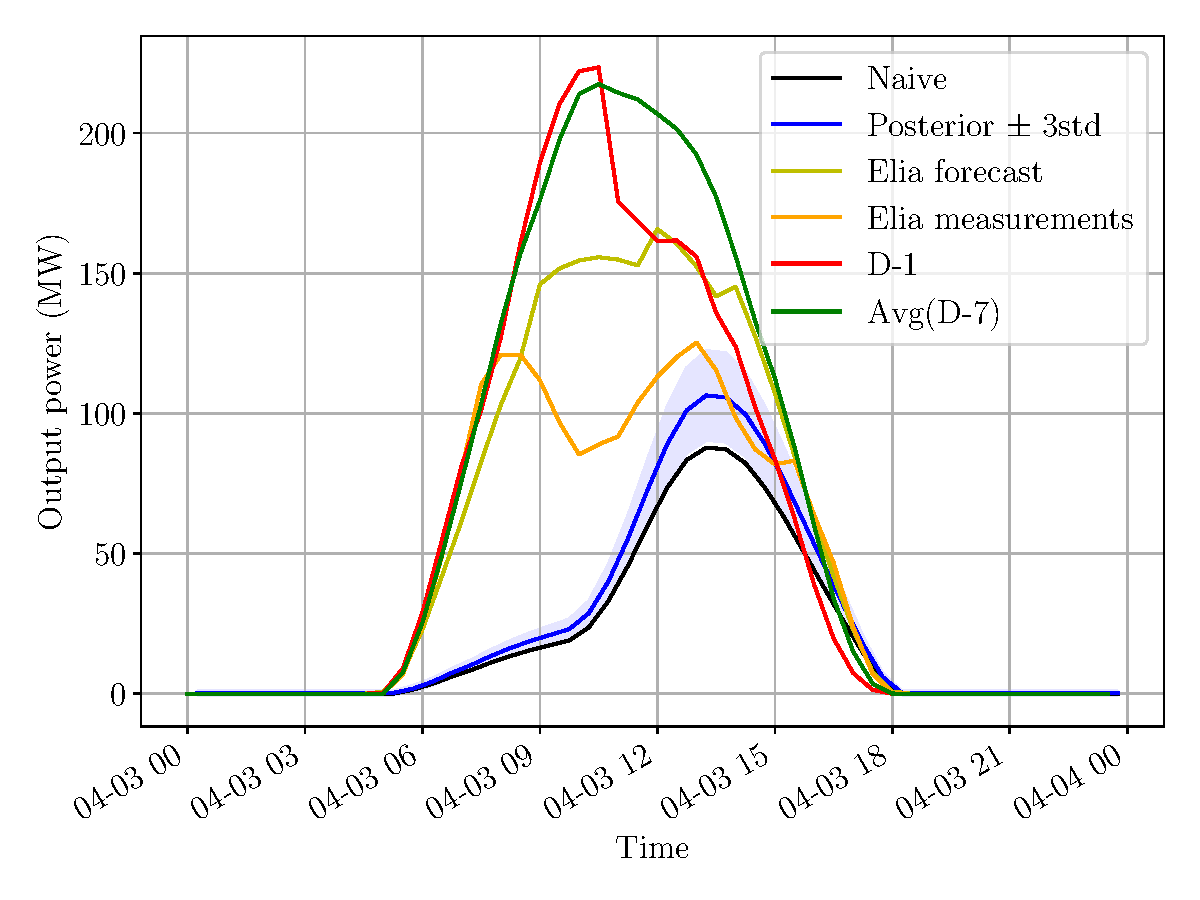
\includegraphics[width=\textwidth]{resources/pdf/solar_provincial (START_FOR 03-04-2020).pdf}
		\caption{Provincial model (using irradiance forecasts).}
		\label{fig:provincial_bad_1}
	\end{subfigure}
	\caption{Samples of inaccurate results with both models (April 3rd 2020) and the baselines.}
	\label{fig:bad_results_april_3rd}
\end{figure}

\begin{figure}[H]
	\centering
	\begin{subfigure}{0.48\textwidth}
		\centering
		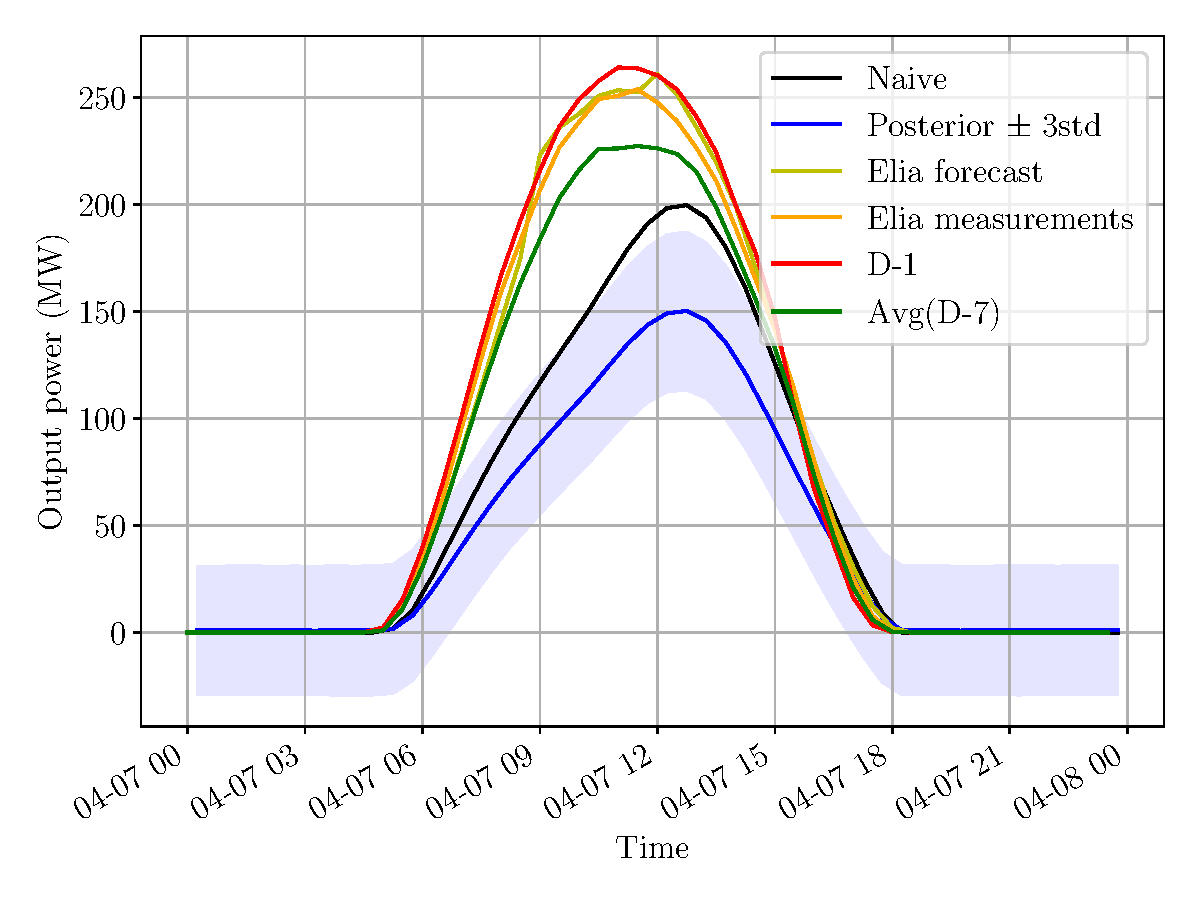
\includegraphics[width=\textwidth]{resources/pdf/solar_panelwise (START_FOR 07-04-2020).pdf}
		\caption{Panelwise model (using irradiance forecasts).}
		\label{fig:panelwise_bad_2}
	\end{subfigure}
	\hspace{0.5em}
	\begin{subfigure}{0.48\textwidth}
		\centering
		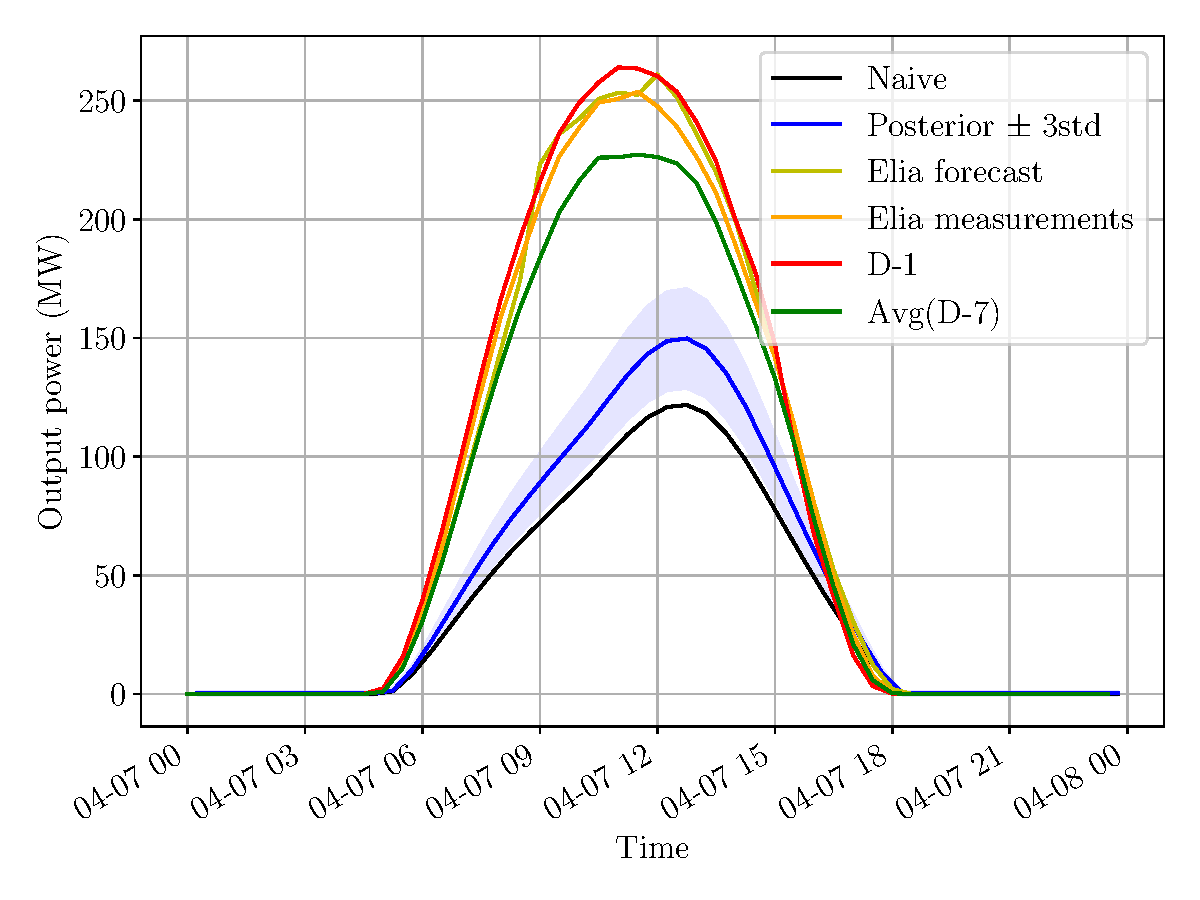
\includegraphics[width=\textwidth]{resources/pdf/solar_provincial (START_FOR 07-04-2020).pdf}
		\caption{Provincial model (using irradiance forecasts).}
		\label{fig:provincial_bad_2}
	\end{subfigure}
	\caption{Samples of inaccurate results with both models (April 7th 2020) and the baselines.}
	\label{fig:bad_results_april_7th}
\end{figure}

Since irradiance forecasts are linked to irradiance measures, in the sense that they are very likely computed from irradiance measures, an alternative to this procedure is to fit to Elia's measures by using an irradiance quantity that would be conditioned on both the irradiance measures and the past irradiance forecasts, assuming that irradiance forecasts represent an unbiased estimate of the true irradiance measures. We conducted tests for the same period (April) but they did not show any improvement, which is why we only decided to mention this alternative without expanding too much.


\subsection{Limitations and possible improvements}
\label{subsec:limitations_solar}
Even though we obtain satisfactory results for the tests conducted on the whole 2019 year (Table \ref{tab:results_2019}), we feel a little bit less satisfied about the results obtained for a \emph{real-life} setting (Table \ref{tab:results_april}), which is quite natural since one uses irradiance measurements while the other one deals with irradiane forecasts.

Nevertheless, this performance loss is something we were prepared for. Indeed, both models rely on simplifying assumptions. 

Our provincial model does not use any information about all the panel installations in the province of Liège. Furthermore, it models the photovoltaic production in a very simple manner, with a normal distribution centered around the product of 4 quantities. Therefore, the only kind of improvements we can expect with respect to the naive model is a re-scale of the original curve. In addition, this production curve (for the naive forecasting model or for the posterior forecasting model) is mainly driven by the irradiance curve. Hence, if the irradiance forecast curve is not representative of the true irradiance that will be measured, it is very likely that the corresponding forecasting models will wrongly estimate the future production. This can be observed on Figure \ref{fig:irradiance_meas_influence} and \ref{fig:irradiance_for_influence}, where the forecast curve is clearly non-representative of the measured power, thus non-representative of the true irradiance measured. Note that this influence is as strong even when we use irradiance measurements.

\begin{figure}[H]
	\centering
	\begin{subfigure}{0.48\textwidth}
		\centering
		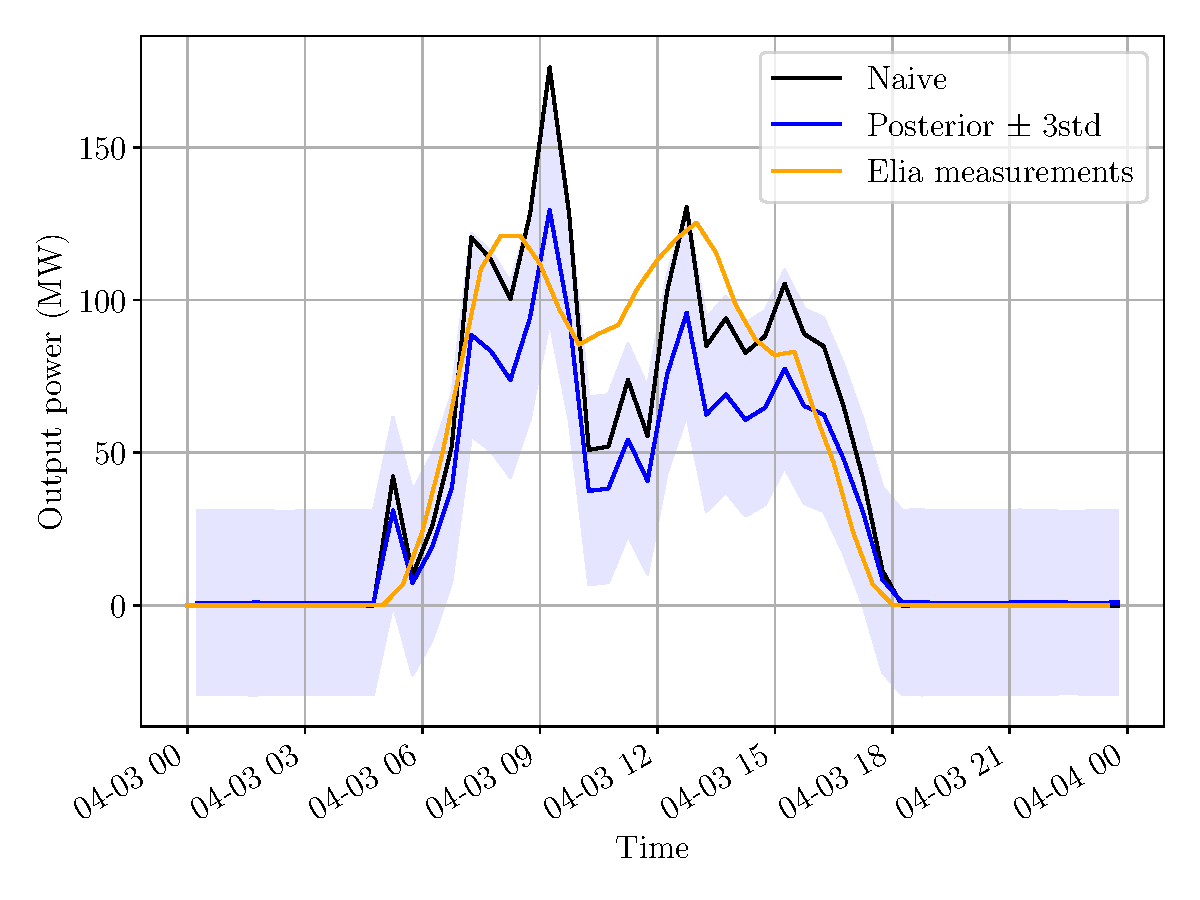
\includegraphics[width=\textwidth]{resources/pdf/solar_panelwise_meas_meas (START_FOR 03-04-2020).pdf}
		\vspace{-0.5em}
		\caption{Panelwise model (using irradiance measurements).}
	\end{subfigure}
	\hspace{0.5em}
	\begin{subfigure}{0.48\textwidth}
		\centering
		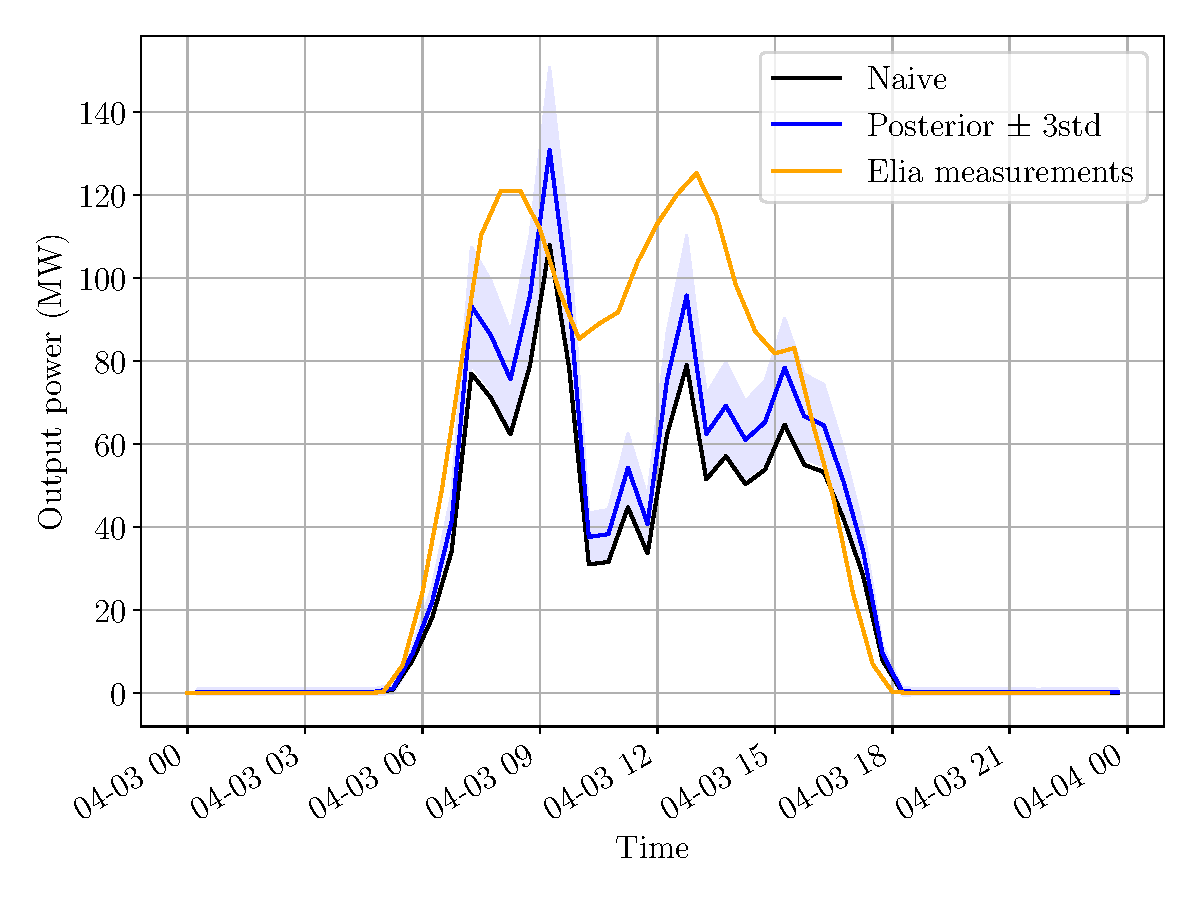
\includegraphics[width=\textwidth]{resources/pdf/solar_provincial_meas_meas (START_FOR 03-04-2020).pdf}
		\vspace{-0.5em}
		\caption{Provincial model (using irradiance measurements).}
	\end{subfigure}
	\hspace{0.5em}
	\begin{subfigure}{0.48\textwidth}
		\centering
		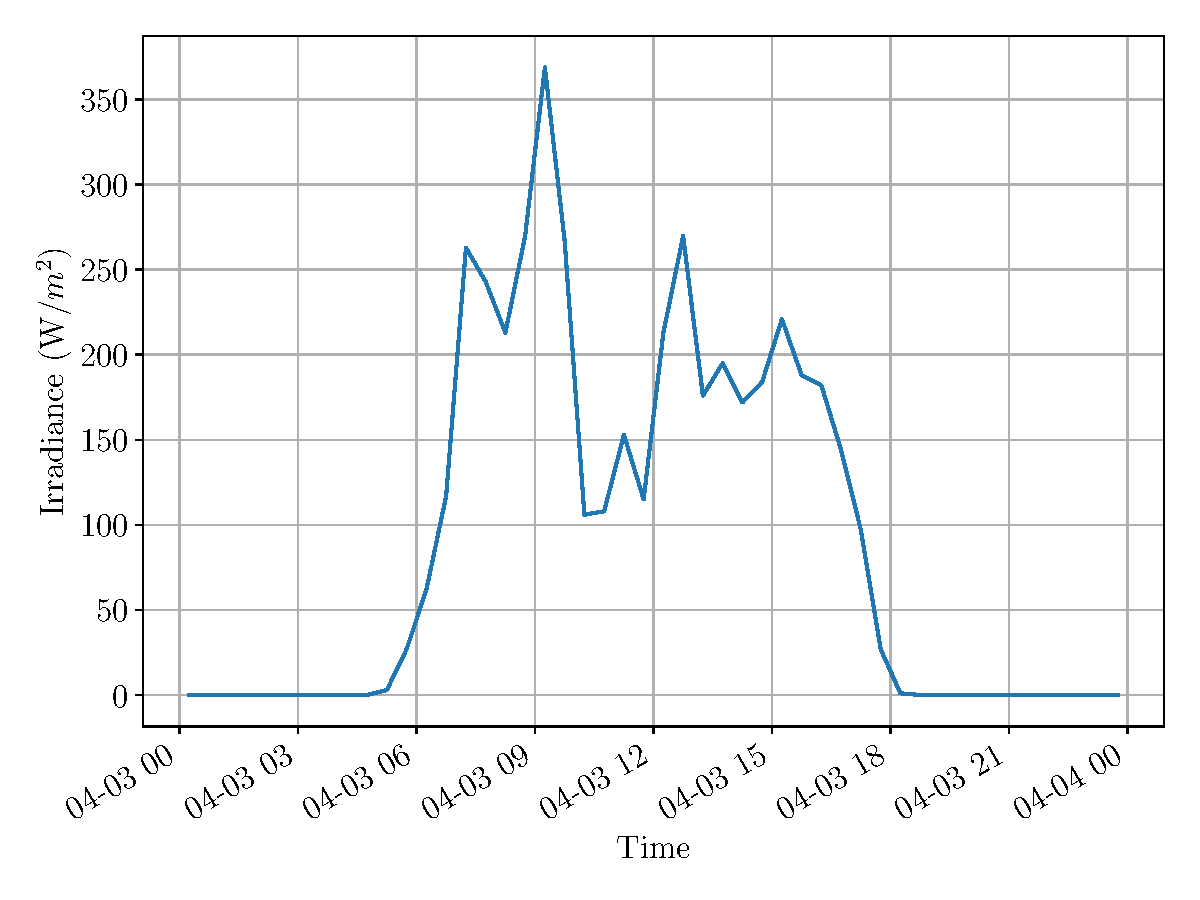
\includegraphics[width=\textwidth]{resources/pdf/irradiance_meas_for (START_FOR 03-04-2020).pdf}
		\vspace{-0.5em}
		\caption{Irradiance measured.}
	\end{subfigure}
	\caption{Influence of the irradiance measures on the predictions.}
	\label{fig:irradiance_meas_influence}
\end{figure}

\begin{figure}[H]
	\centering
	\begin{subfigure}{0.48\textwidth}
		\centering
		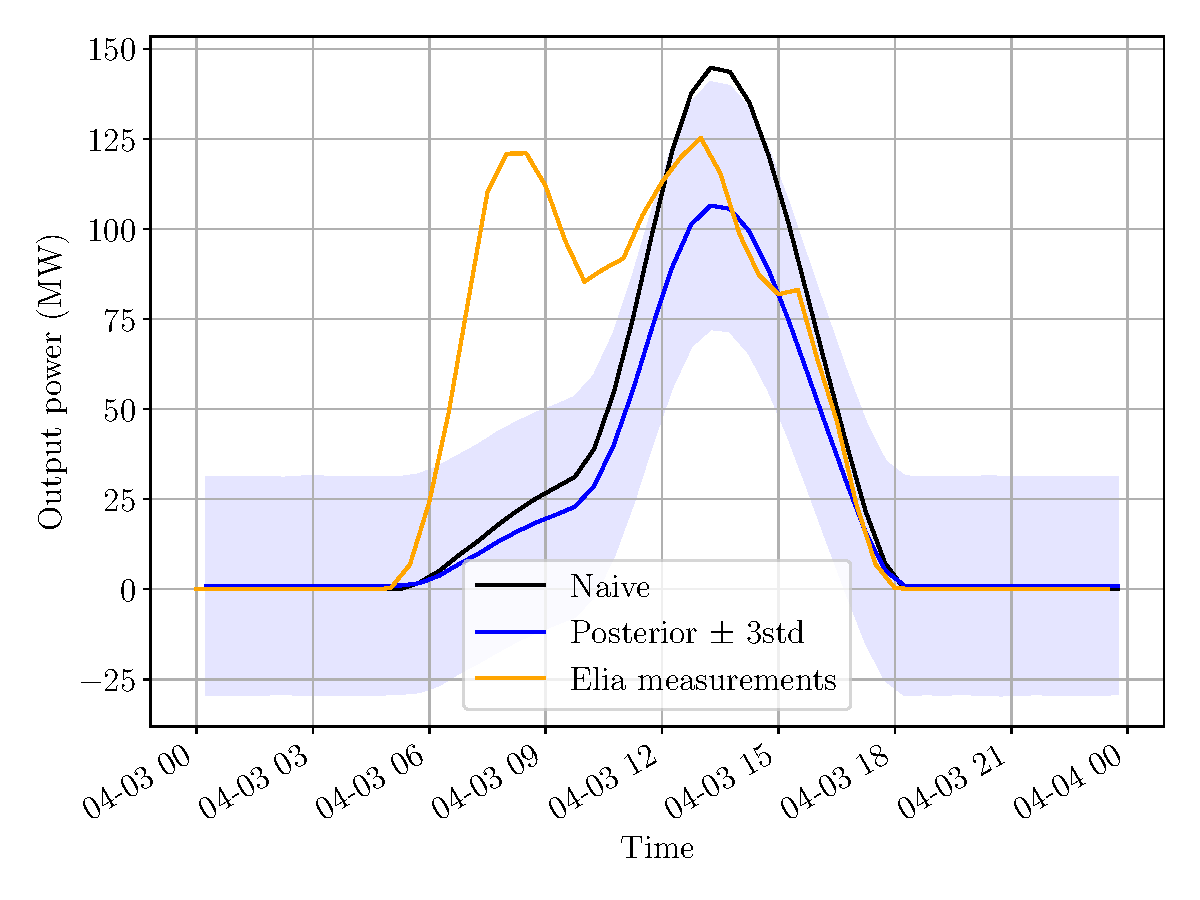
\includegraphics[width=\textwidth]{resources/pdf/solar_panelwise_meas_for (START_FOR 03-04-2020).pdf}
		\vspace{-0.5em}
		\caption{Panelwise model (using irradiance forecasts).}
	\end{subfigure}
	\hspace{0.5em}
	\begin{subfigure}{0.48\textwidth}
		\centering
		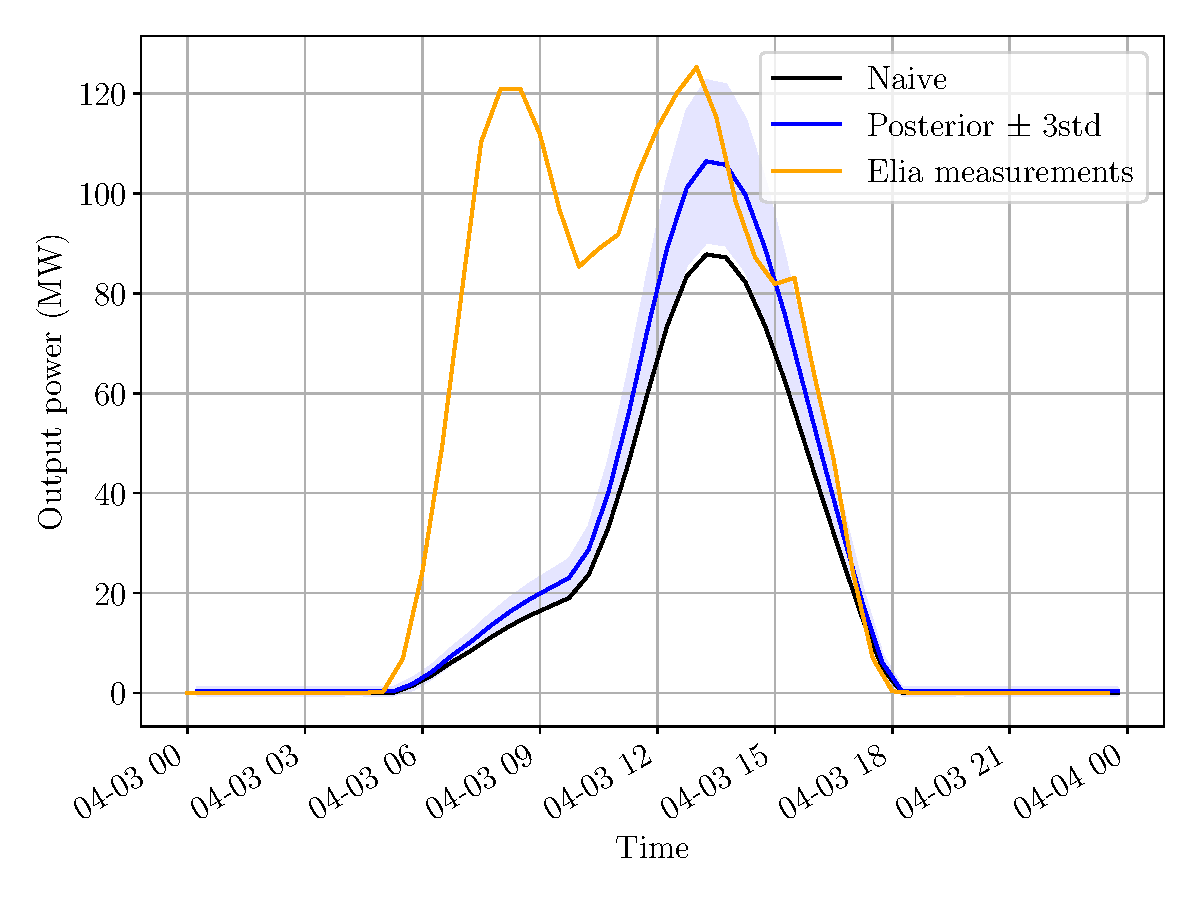
\includegraphics[width=\textwidth]{resources/pdf/solar_provincial_meas_for (START_FOR 03-04-2020).pdf}
		\vspace{-0.5em}
		\caption{Provincial model (using irradiance forecasts).}
	\end{subfigure}
	\hspace{0.5em}
	\begin{subfigure}{0.48\textwidth}
		\centering
		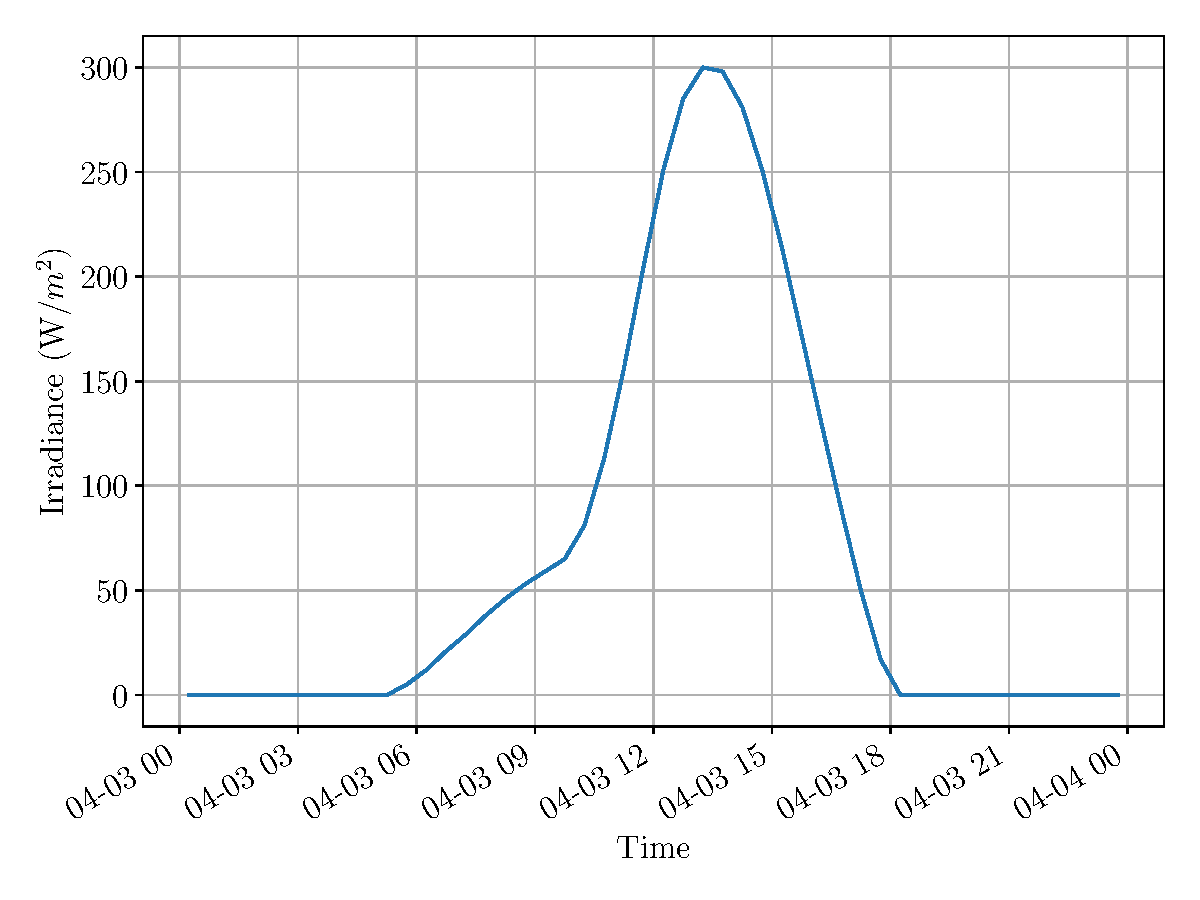
\includegraphics[width=\textwidth]{resources/pdf/irradiance_for_for (START_FOR 03-04-2020).pdf}
		\vspace{-0.5em}
		\caption{Irradiance forecasted.}
	\end{subfigure}
	\caption{Influence of the irradiance forecasts on the predictions.}
	\label{fig:irradiance_for_influence}
\end{figure}


Furthermore, we only retrieve irradiance data at a single location, which we chose to be the city of Liège\footnote{Coordinates: (\SI{50.6326}{\degree}, \SI{5.5797}{\degree})}. This restriction thus naturally implies that the irradiance curve will, most of the time, not be of the same shape as the measured power.

As far as our panelwise model is concerned, it is somehow more sophisticated since it considers panel-specific characteristics: its location (latitude and longitude), its estimated area, azimuth, etc. Therefore, it should be more precise about the produced power. It is the case for the panelwise model applied to ULiège, as could already have been seen on Figure \ref{fig:sart_tilman}. This is quite logical since we had access to very accurate irradiance data and technical specifications. Note that no uncertainty was introduced in the ULiège model because we knew exactly the number of panels, their areas, azimuths, etc. 

It is no longer the case when we extend this model to the whole province, as can be seen from Figure \ref{fig:panelwise_bad_1} and \ref{fig:panelwise_bad_2}. Indeed, the estimated azimuths and areas are, as their name indicates, \emph{estimates}; hence less reliable. Yet, one could have expected consistently more accurate results than for the provincial model. This is not true, since we use the exact same irradiance data. Therefore, we also have the restriction of a single irradiance location. Note that, even more than for the provincial model, it would have been unfeasible to request irradiance data at each panel location, as there are so many in the province of Liège.

A way of partly solving this issue could have been the following: assuming we could request irradiance data at multiple sites, we could try and \emph{aggregate} (in some sense) the panels locations into a much reduced number of locations, according to their coordinates. Obviously, when computing the solar angles, we would still consider each panel's true coordinates. Then, we could compute each installation's output power according with their corresponding irradiance, chosen according to their closest aggregate location. Although we did not try this alternative (which we couldn't because of the API limitations), we feel that this would very likely help our model.

\newpage
\part{Wind power}

\section{Wind power production}
\label{sec:wind_power}

\subsection{Overview of wind power forecasting}

	\paragraph{Classification of wind forecasting problems}

	In wind power forecasting, one can be interested in different problems:
	\begin{itemize}
		\item Very-short-term or immediate-short-term (a few hour ahead);
		\item Short-term or medium-term (few hours to several days);
		\item Long-term (multiple days ahead);
	\end{itemize}
	Each of these problems answers different needs (load balancing, power production planning, long-term power needs prognostication, etc), but above all, each of these problems makes use of different mathematical, statistical or algorithmic tools. Our project addresses the day-ahead task, falling into the short-term category.

	Below, we will discuss the most appropriate approach to use among the classical approaches in wind power forecasting.
	
	\paragraph{Classical approaches in wind power forecasting}
		
	From different reviews of wind power forecasting \parencite{sweeney2019future, messner2020windpower}, we have identified the following approaches in this field.

	\begin{enumerate}[label=\arabic*]

		\item \textbf{Physical modeling}: based on Numerical Weather Prediction (NWP), the model aims at outputting the power produced by one power plant using the power plant characteristics (wind turbine power curves, surface roughness and obstacles, terrain wake, hub heights, even the wind farms wake effect on themselves is taken into account in recent works). These approaches are said to be very computationally expensive, and quite hard to apply on very large scale situation such as the Wallonia which is constituted of 67 power plants. 

		\item \textbf{Statistical modeling}
		\begin{enumerate}[label=\alph*.]
			\item On the very short term: \emph{time series based forecasting}: the NWP data is not used, only the power time series is used to make the prediction. This approach is said to be hard to beat on 4 to 6 hours ahead predictions (very short term).

			\item On the longer term: \emph{post processing of NWP}: the temporal aspect is not considered. The power predictions are based on NWP. Roughly, this approach aims at mimicking the physical model when some information are missing such as the surface roughness and terrain wake effect for each power plant. 
		\end{enumerate}

		\item \textbf{Hybrid method}: uses \emph{post processing of NWP} \textbf{and} \emph{of physical modeling}.
	\end{enumerate}

	The most promising and adapted approach seems to be the \emph{post processing of NWP}. Indeed, we address the day-ahead forecasting task, weather data and aggregated power measurements are available, and power plant physical characteristics are not available to build a complete physical model.

    \paragraph{Physical model}
	However, a simple physical model has been built as a baseline. Unfortunately, it performs poorly, as can be seen on figure \ref{fig:wind_phys}. This model uses the power curves retrieved from the \emph{wind turbine models} website \parencite{wind-turbine-models}, or, when not available, builds naive theoretic power curve from the cut-in, cut-out and rated wind speed, using the well known cubic relation, as can be seen on figure \ref{fig:wind_pc} and \ref{fig:wind_pc_theoretic}. This is done for the 35 models of wind turbines present in Wallonia. The automatic retrieval of wind turbines characteristics (power curve, cut-in, cut-out and rated wind speed) is done in \texttt{cache/wind\_farms.py}.

	Then, it computes the power produced at each wind turbine, using as input the wind speed measured at the power plant of this wind turbine. Finally, all results are aggregated. The implementation of this simple physical model can be found in \texttt{misc/wind\_phys\_model.py}. On the month of March 2020, the MAE (mean absolute error) was of \SI{355.16}{MW}. 

	\begin{figure}[H]
		\centering
		\begin{subfigure}[t]{0.48\textwidth}
			\centering
			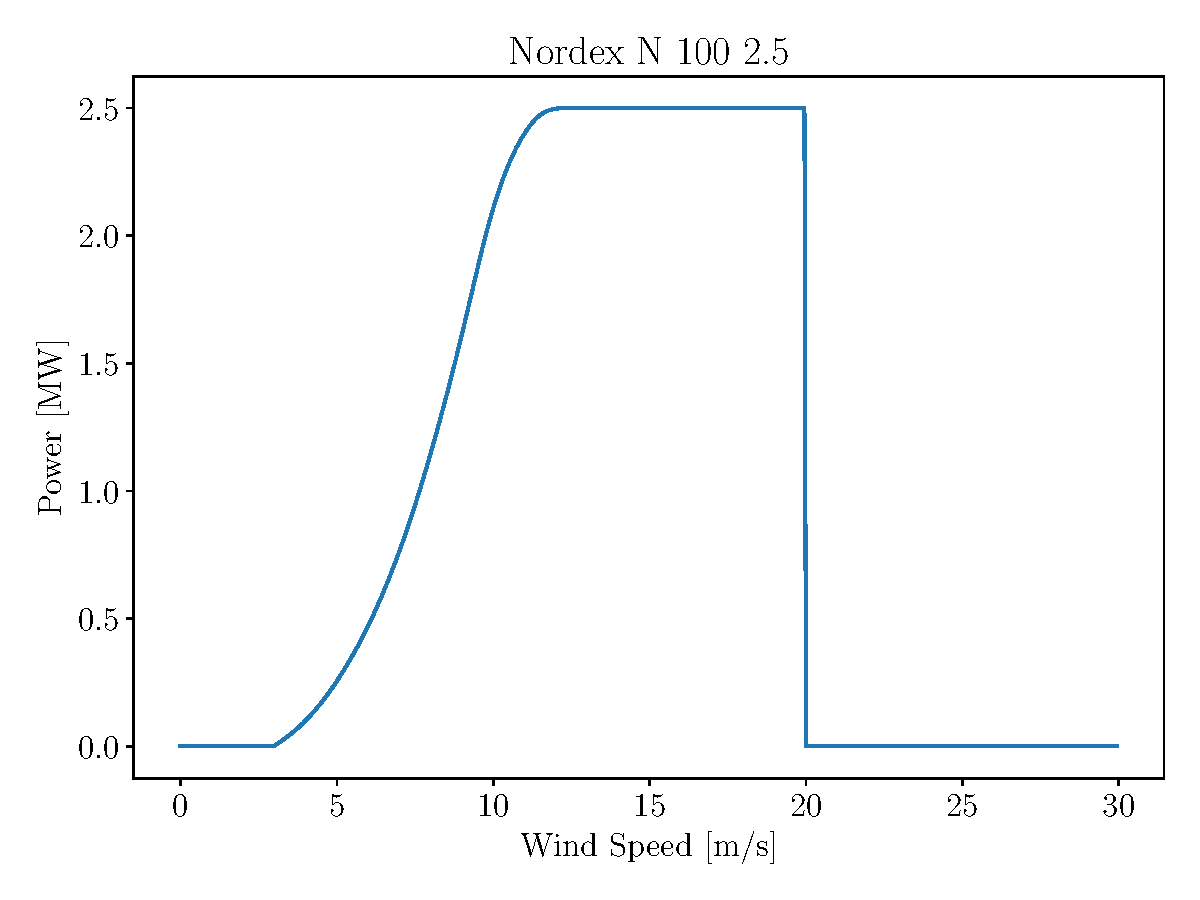
\includegraphics[width=\textwidth]{resources/pdf/wind_pc.pdf}
			\caption{Power curve}
			\label{fig:wind_pc}
		\end{subfigure}
		~ 
		\begin{subfigure}[t]{0.48\textwidth}
			\centering
			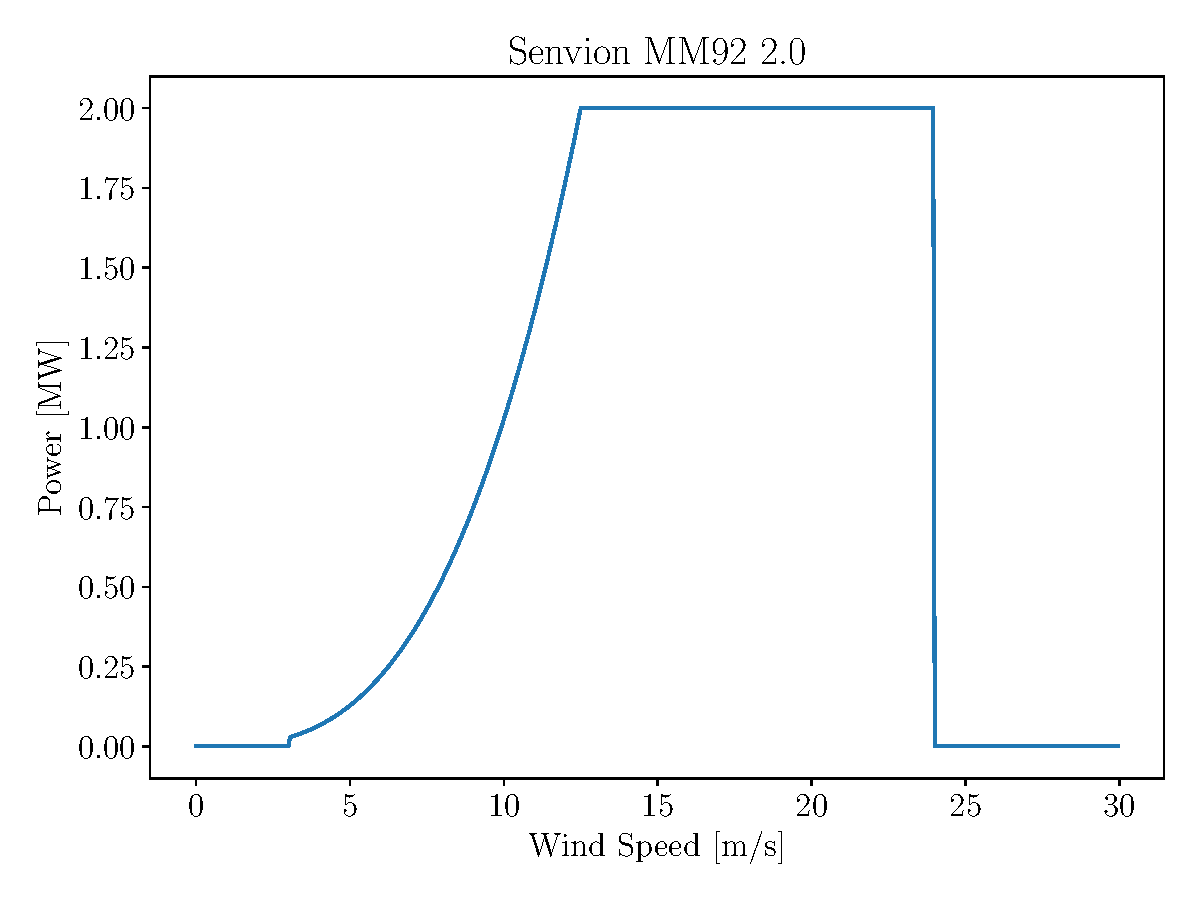
\includegraphics[width=\textwidth]{resources/pdf/wind_pc_theoretic.pdf}
			\caption{Theoretic power curve}
			\label{fig:wind_pc_theoretic}
		\end{subfigure}
		\caption{Examples of power curves}
	\end{figure}

	\begin{figure}[H]
		\centering
		\begin{subfigure}[t]{0.48\textwidth}
			\centering
			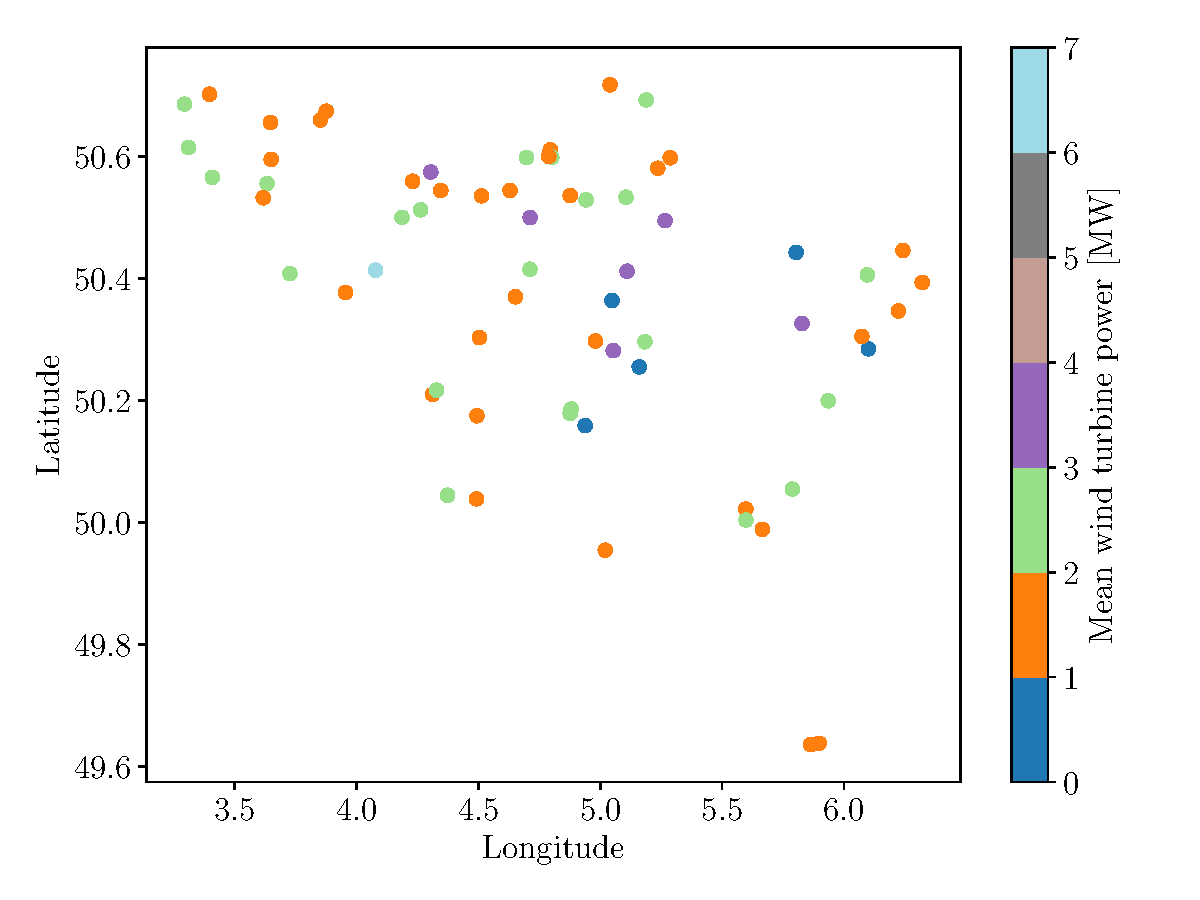
\includegraphics[width=\textwidth]{resources/pdf/wind_farms.pdf}
			\caption{Wind power plants in Wallonia}
			\label{fig:wind_farms}
		\end{subfigure}
		~
		\begin{subfigure}[t]{0.48\textwidth}
			\centering
			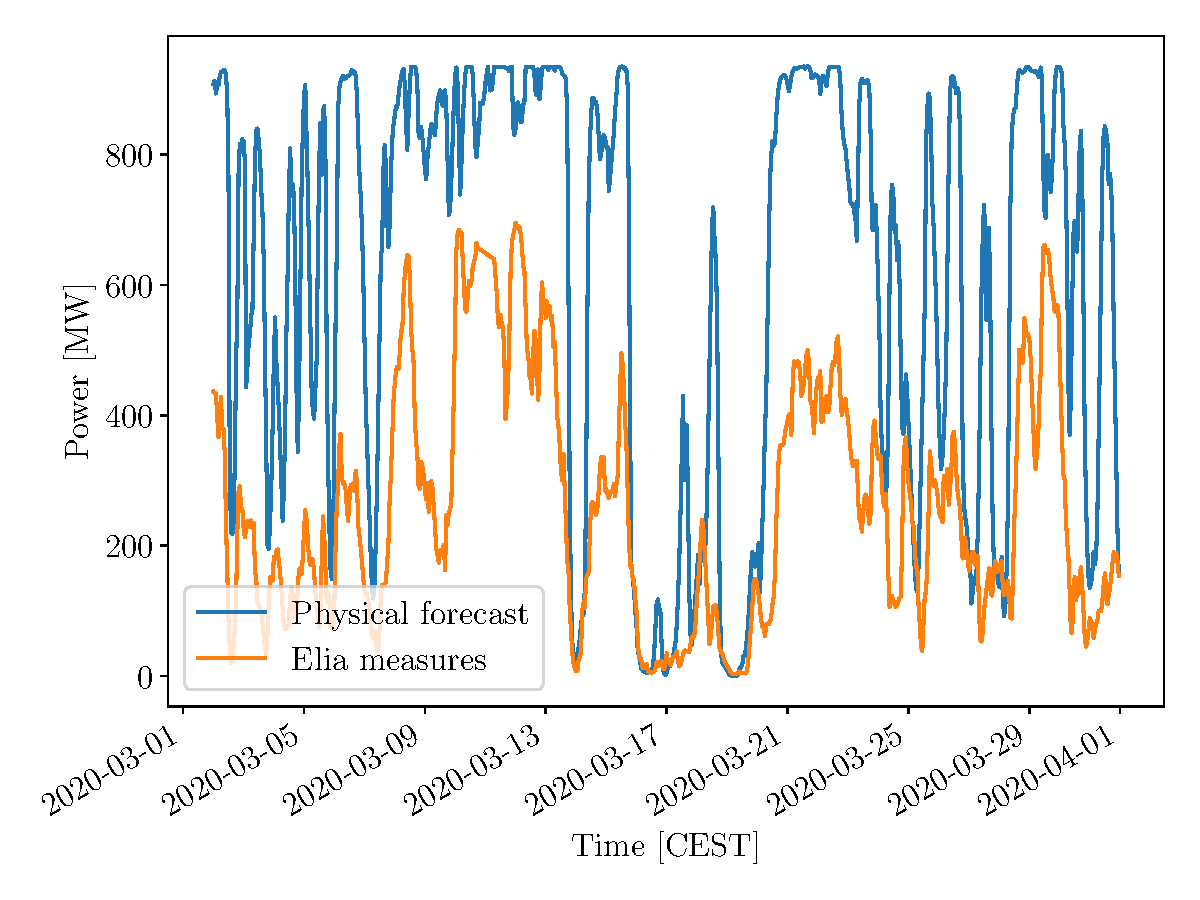
\includegraphics[width=\textwidth]{resources/pdf/wind_phys.pdf}
			\caption{Physical model forecast example}
			\label{fig:wind_phys}
		\end{subfigure}
		\caption{Wind power plants location and physical model}
	\end{figure}
	
\subsection{Data and computation flow}

	\subsubsection{Data}

	Several source of data were available and have been used in the wind forecast computation:
	\begin{itemize}
		\item \textbf{List of wind turbines} in Wallonia \parencite{spw-energie}: list of all wind turbines in 2018 and projects for 2019. This data can be visualized on figure \ref{fig:wind_farms} (aggregated by wind power plants). For each wind turbine, the following data is available:
		\begin{itemize}
			\item Location (latitude and longitude);
			\item Power plant unique name;
			\item Wind turbine model reference (brand - type - nominal power).
		\end{itemize}
		\item \textbf{Wind turbine models characteristics} \parencite{wind-turbine-models}
		\begin{itemize}
			\item Cut-in, cut-out and rated wind speeds;
			\item Power curve.
		\end{itemize}
		\item \textbf{Wind power measures and forecast for Wallonia} \parencite{elia-wind}: measures and day-ahead forecast in \si{\mega\watt} every \SI{15}{\minute}
		\item \textbf{Wind weather measures and forecast} \parencite{darksky}: one 7-measure every hour at any location requested.
		\begin{itemize}
			\item Wind speed, wind gust, wind bearing, temperature, humidity, pressure, air density.
		\end{itemize}
	\end{itemize}
	
	As can be seen here, no data is available to evaluate the wind power production forecast at the Liege province level. Thus, the whole wind forecasting task is performed \emph{at the regional level}.

	\subsubsection{Computation flow}

	The figure \ref{fig:wind_computation_flow} helps clarifying the way data has been used in the computation of the forecast.

	As the NWP post-processing approach has been selected, the first step was to build a learning set on which to build models. As can be seen from figure \ref{fig:wind_computation_flow}, the learning set is built in the following way:
	\begin{itemize}
		\item Computation of the mean locations of the 67 wind power plants from the \emph{SPW Energie} data (\texttt{cache/wind\_farms.py})
		\item Retrieval of 2.25 years of 7-dimensional weather measures at the 67 locations from \emph{Darksky} (\texttt{cache/wind\_weather.py})
		\item Retrieval of 2.25 years of total wind power measures in Wallonia Region from \emph{Elia} (\texttt{cache/wind\_power.py})
		\item Union of the two sets of data: weather (input) and power (output) into a learning set, with the measures of elia being averaged per hour, constituting a \emph{weather measures} learning set (\texttt{cache/wind\_ls.py})
	\end{itemize}

	In parallel, from April 5th, a \emph{weather forecast} test set is built. It is constituted of weather forecast as input instead of weather measurements. Indeed, doing so will allow us to quantify the loss in performance when using our model in real conditions (\textit{i.e.} on forecast). As no data is available for past weather forecast, we had to request it each day (at 11 o'clock) for the next day and store it. This explains why this test set is unfortunately available from the 5th of April only.\footnote{As will be discussed later, the forecasting turned out to be unusable because the considered time period showed signs of non representability with respect to the usual wind power.}

	Then, the model is built using a part of the learning set as train set, and evaluated on weather measures using another part of the learning set set. Finally, its performance in real conditions is evaluated using the \emph{weather forecast} test set.

	As most of the steps of this computation flow are very slow and unreliable (rely on external API), we have decided to use a cache-based approach. It means that each step uses the data that has been cached by its parents in the graph, and never asks them to re-compute it in live. For most of the data, it is not necessary to refresh the cache very often.

	\begin{figure}[H]
		\centering
		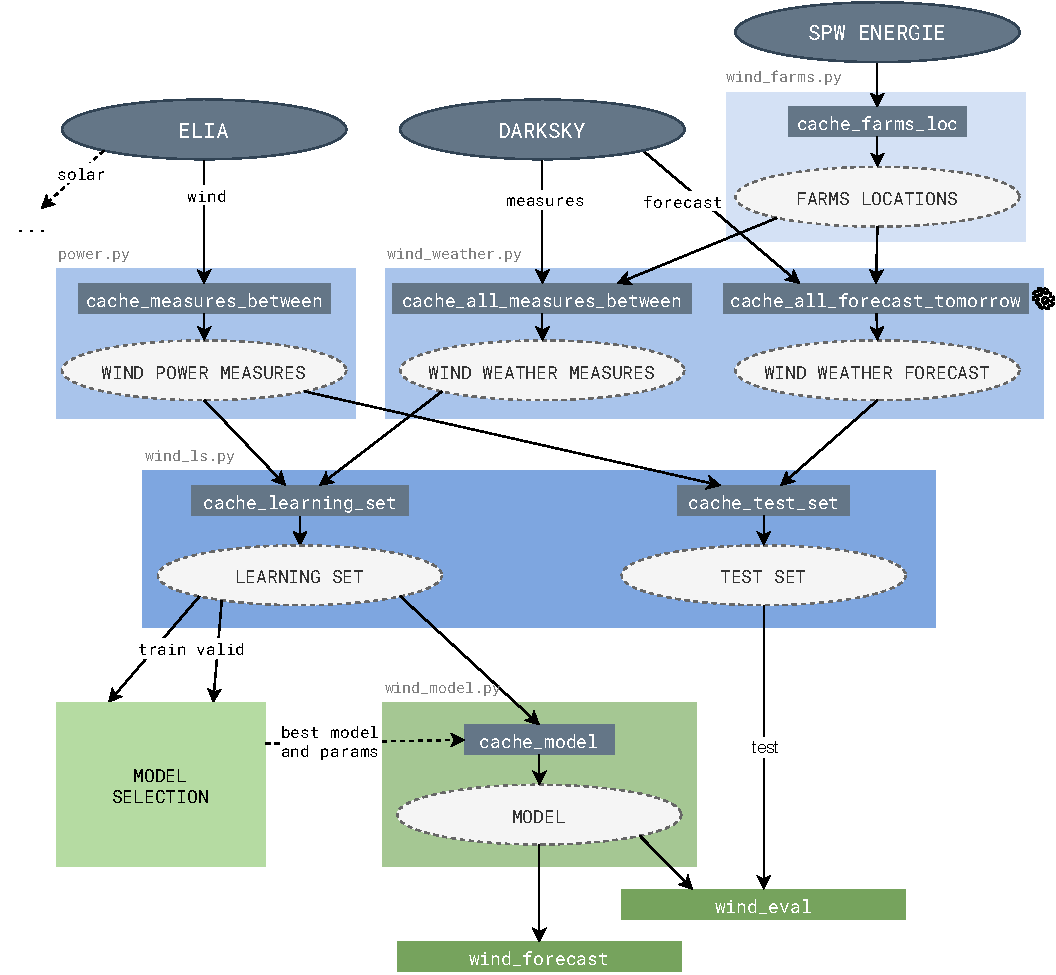
\includegraphics[width=.8\textwidth]{resources/pdf/diagram_wind.pdf}
		\caption{Wind forecast computation flow}
		\label{fig:wind_computation_flow}
	\end{figure}


	\subsubsection{Feasibility}

	The above mentioned computation flow has allowed constituting a learning set of 67 7-dimensional inputs, resulting in 469 inputs, for one output: the wind power in Wallonia. The feasibility of the regression has quickly been concluded, by running a quick model (random forest) on only one feature (wind speed measure in Namur) to predict the output. This model already achieved a MAE (mean absolute error) below \SI{100}{\mega\watt}, whereas the maximum wind power observed in Wallonia, according to \emph{Elia}, is \SI{727}{\mega\watt}.

	Furthermore, as can be seen on figure \ref{fig:wind_missingness}, the missingness on the 469 variables is really moderate, with almost only one chunk of 3 months that is not represented. If the wind present seasonal patterns, the fact that 2.25 years of data has been retrieved will solve the problem of these three months.
	
	\begin{figure}[H]
		\centering
		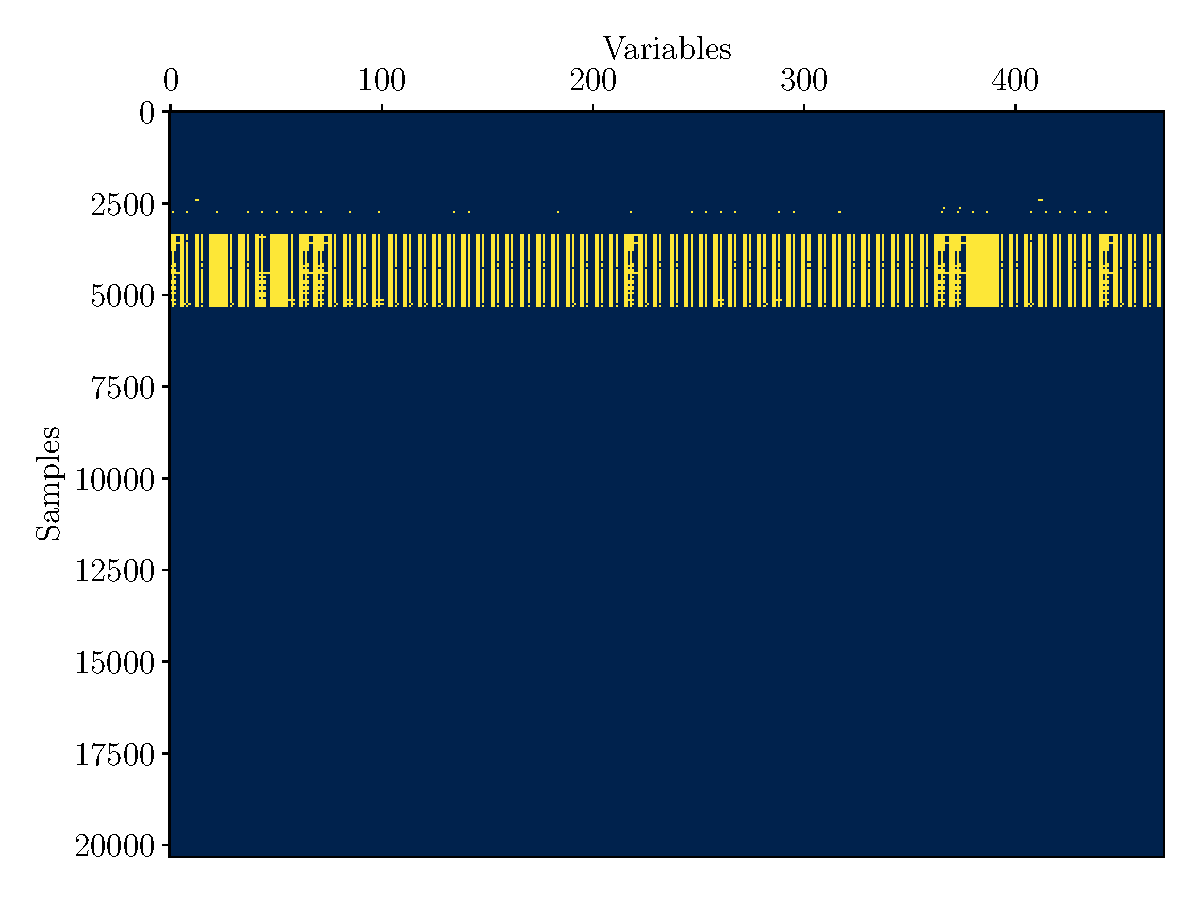
\includegraphics[width=.5\textwidth]{resources/pdf/wind_missingness.pdf}
		\vspace{-1em}
		\caption{Missingness in the learning set (2069 NA corresponding to \SI{0.024}{\percent})}
		\label{fig:wind_missingness}
	\end{figure}

	Finally, by looking at figure \ref{fig:wind_wallonia_pc}, which corresponds to a kind of Wallonian power curve, we can see that a certain relation seems to exist between the mean wind speed at the 67 locations and the wind power in Wallonia.

	\begin{figure}[H]
		\centering
		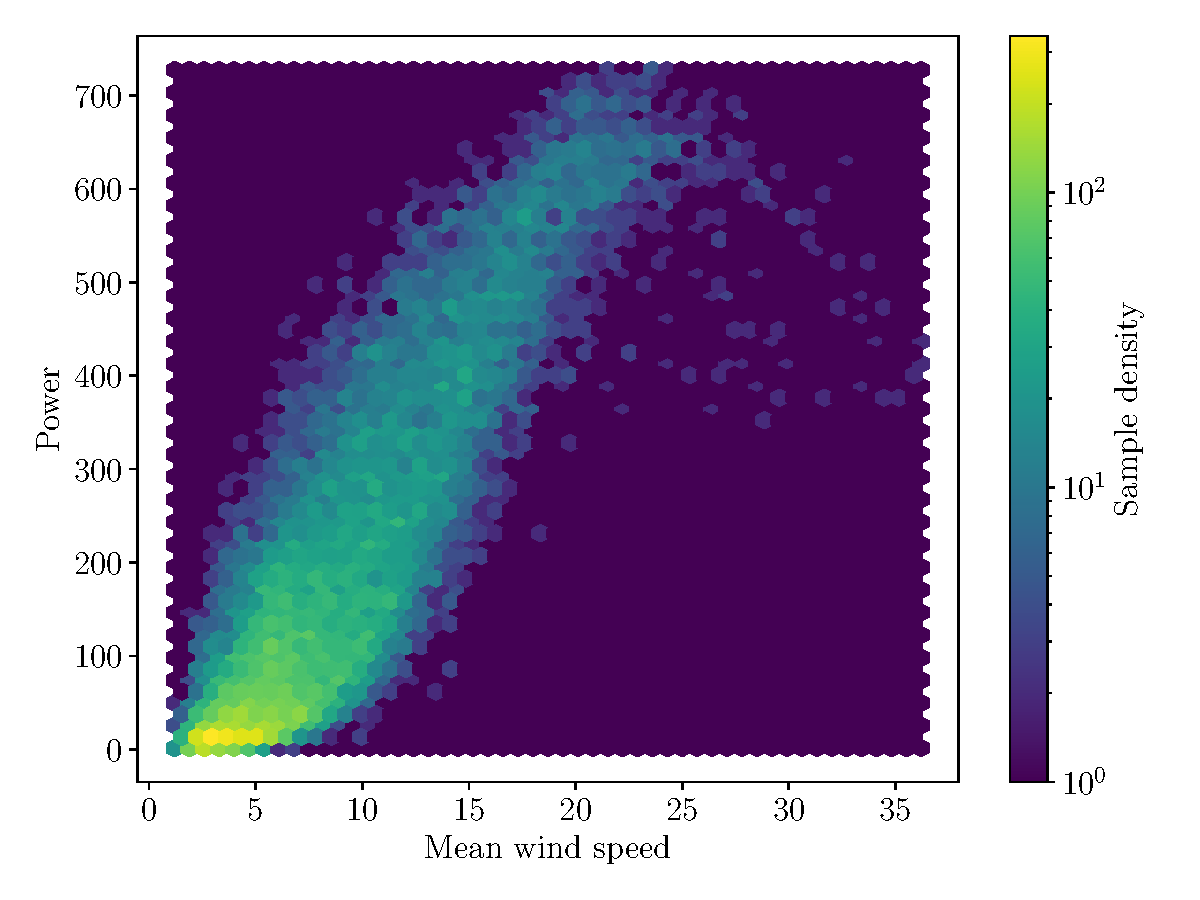
\includegraphics[width=.8\textwidth]{resources/pdf/wind_wallonia_pc.pdf}
		\vspace{-1em}
		\caption{Learning set sample density with respect to the total power and the mean wind speed at the 67 wind power plants location}
		\label{fig:wind_wallonia_pc}
	\end{figure}

	\subsubsection{Feature selection}
	After having identified that models such as random forests and extra trees performed very well on the whole learning set (469 inputs), we have considered feature selection, since some of the weather measurements are certainly not relevant to the problem.

	To assess the feature importances, we have used the mean impurity reduction in the extra trees forest for each variable (mean variance reduction in the case of regression). This resulted in the explicit results of figure \ref{fig:wind_fi}. The feature importances of each of the 469 variables are grouped by type of variable (wind speed, temperature, etc) and the density of feature importances for each type of variable has been estimated on the violin plot.

	As can be clearly seen from the figure, the two most important features are the wind speed and wind gust, which totally makes sense, the other variables having negligible importance. We thus decided to keep these 2 types of variables only. Indeed, with mean feature importances of respectively \SI{0.88}{\percent} and \SI{0.52}{\percent}, the 134 variables constituted by these two type of features gather around \SI{93.8}{\percent} of the mean impurity reduction.

	Furthermore, by comparing the results obtained on unseen data, especially when the train-test split is not shuffled, the algorithms generalized better when working only on these two types of variables than when working with all of them. This feature selection have thus allowed overfitting reduction.

	\begin{figure}
		\centering
		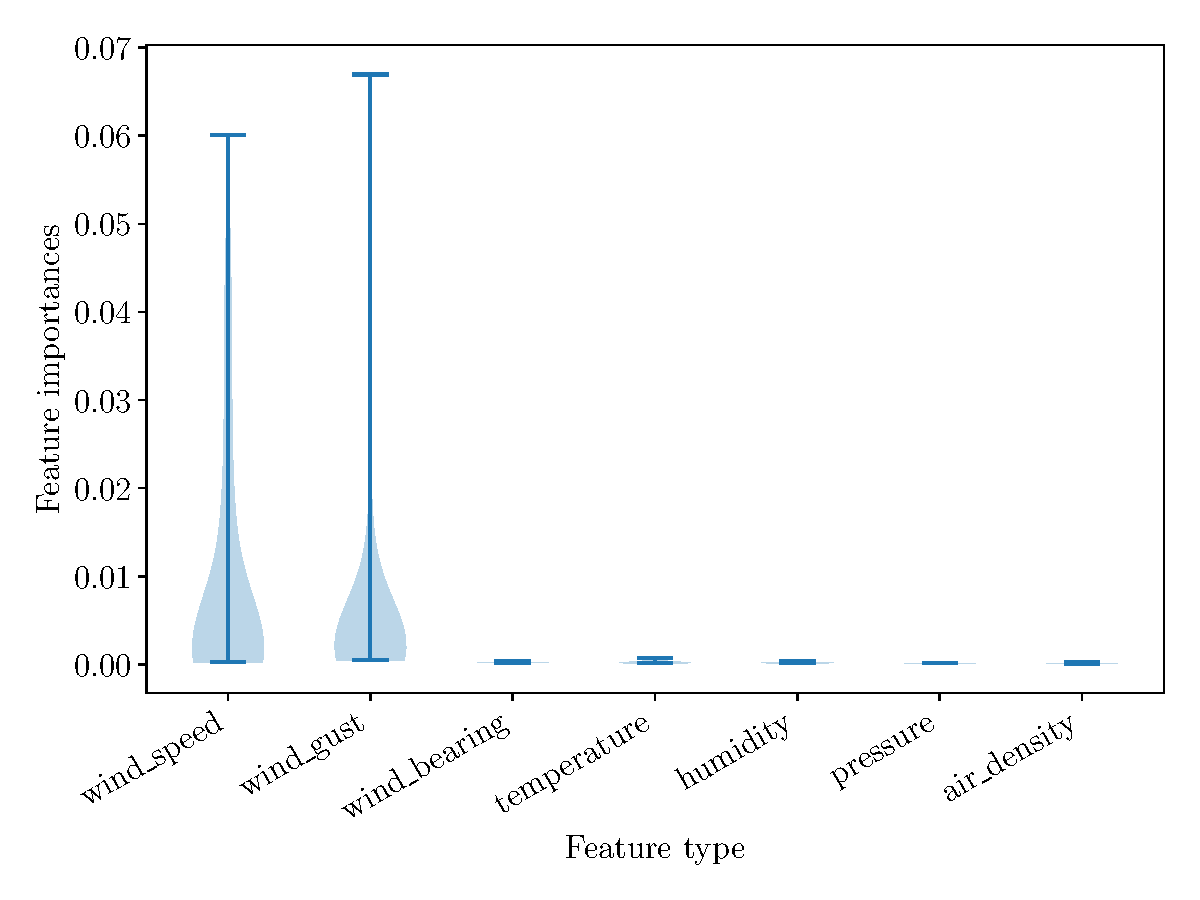
\includegraphics[width=0.8\textwidth]{resources/pdf/wind_fi.pdf}
		\vspace{-1em}
		\caption{Feature importances distribution with respect to the type of feature}
		\label{fig:wind_fi}
	\end{figure}


\subsection{Model selection}

	The model selection has been performed on the \emph{weather measures} learning set, without using any data coming from the \emph{weather forecast} set. This set has been shuffled and divided in three parts: 
	\begin{itemize}
		\item LS:
		\begin{itemize}
		    \item Train set (50\%);
		    \item Validation set (25\%);\\
		\end{itemize}
		\item{TS:}
		\begin{itemize}
		    \item Test set (25\%);
		\end{itemize}
	\end{itemize}
	We can already note that this way of splitting the learning set will probably lead to overly optimistic results because of the shuffling. Indeed, the wind power and wind weather are highly correlated from one hour to another. Fortunately, the \emph{weather forecast} test set whose construction has been discussed above will fix this problem.
	

	\subsubsection{Supervised learning method selection}

	A certain number of supervised learning methods have been experimented. The performance of each model has been estimated by computing the MAE on the validation set for several combination of parameters for each model. All models have yielded validation set MAE between \SI{31}{\mega \watt} and \SI{33}{\mega \watt}, for all parameters combinations. The best scores obtained on the validation set are gathered in table \ref{tab:wind_sl_methods}.
	
	\begin{table}[H]
		\centering
		\resizebox{\textwidth}{!}{%
		\begin{tabular}{|l|c|c|c|}
		\hline
			\textbf{Supervised Learning Method} & \textbf{MAE} & \textbf{nMAE} [\si{\percent}] & \textbf{Time}\footnotemark[\value{footnote}] [\si{\second}] \\ \hline
			Random Forest (500 trees) & 32.24 & 4.43 & 68 \\ \hline
			Extra Trees (500 trees) & 31.05 & 4.27 & 24 \\ \hline
			Extra Trees (500 trees, ‘sqrt’ max features) & 32.59 & 4.48 & 3 \\ \hline
			Extra Trees (500. ‘sqrt’ max features. ‘mae’ criterion) & 32.76 & 4.50 & 248 \\ \hline
			MLP (hidden layers: 1024, 1024, 512, 128, 64) & 31.99 & 4.40 & 430 \\ \hline
			Gradient Boosting (1000 trees, .1 learning rate, .7 subsample) & 32.29 & 4.44 & 160 \\ \hline
		\end{tabular}}
		\caption{Best scores on validation set and computation times (MAE and MQL are expressed in \si{\mega\watt})}
		\label{tab:wind_sl_methods}
	\end{table}
	
	\footnotetext{Model trained with 4 threads available (for the extra trees), on a \SI{2.9}{\giga\hertz} Intel Core i5 double core with \SI{8}{\giga o} of \SI{2133}{\mega\hertz} LPDDR3 RAM\label{notetime}}
	\stepcounter{footnote}

	Even if we can't assess the performance of each of these models on their validation set scores (having tested lots of parameters combination, one could be low by a stroke of luck), they leave use confident on the fact that no supervised learning method should be that much better than the others (see distribution of scores obtained on all the considered hyper-parameters in notebook \texttt{wind\_models.ipynb}: all between \SI{31}{\mega\watt} \SI{33}{\mega\watt}).

	We decided to focus our selection of supervised learning method on two well known family of supervised learning algorithms: tree ensembles and tree boosting, namely the Extra Trees and the Gradient Boosting methods. We will immediately focus on the MSE minimization criterion instead of MAE, since it is far more computationally efficient for datasets as large as the one that we use (around \num{18000} samples). Moreover, the MAE criterion tested on extra trees (because they are the fastest method) has not shown better performance in terms of MAE on the validation set.

	\subsubsection{Quantile predictions}

	In addition to the traditional estimation of the conditional expectation $\mathbb{E}\{Y|X\}$, we would like to have confidence intervals. 

	The gradient boosting method can be adapted straightforwardly, using an appropriate quantile loss in the boosting procedure. However, three separate trees will have to be built to predict the lower quantile, the upper quantile (using the quantile loss), and the expectation estimation (using a least square loss for this one).

	For the extra trees, another approach is used, allowing to build a single forest. The idea is to have a higher minimum number of sample per leaf (for exemple, 10). The trees are built as usual, but instead of keeping only information such as the mean and variance for each leaf, we keep information on all the target values that have ended up in each leaf. 

	Then, at prediction time, a certain input will end up in $T$ leaves (one leaf per tree), and its $q$-quantile can be estimated by interpolating between the all the samples that are in these $T$ leaves, several interpolation methods are possible (\href{https://en.wikipedia.org/wiki/Percentile#The_linear_interpolation_between_closest_ranks_method}{Wikipedia — Percentile Interpolation}). We have used the library \texttt{scikit-garden} that implements this by aditionnaly weighting the samples in each of the $T$ considered leaves by the proportion of train samples that have ended up in each leaf \parencite{meinshausen2006quantile}. Of course, this method is thus far more computationally expensive at prediction time.

	Two wrappers have been built to use these two models with a single \texttt{fit} and a single \texttt{predict} method, they can be found in the python module \texttt{cache/quantile\_models.py}.

	\subsubsection{Hyper-parameters tuning}

	The hyper-parameters have been tuned by using 4-folds cross-validation on the LS (train and valid). The parameters having lead to the minimum mean MAE on the 4-folds are kept. These hyper-parameters are the following:
	\begin{itemize}
		\item Quantile Extra Trees: \num{1 000} estimators, minimum number of samples required to split: \num{10}, number of features to consider when looking for the best split: all.
		\item Quantile Gradient Boosting: \num{1 000} estimators, learning rate: \num{0.1}, number of features to consider when looking for the best split: all, subsample: \num{0.7}.
	\end{itemize}


\subsection{Results}

	The two models performances are then assessed by computing the following metrics:
	\begin{itemize}
		\item MAE (mean absolute error);
		\item nMAE (normalized mean absolute error);
		\item nRMSE (normalized root mean squared error);
		\item MQL10 (mean quantile loss for \num{10}\textsuperscript{th} quantile);
		\item MQL90 (mean quantile loss for \num{90}\textsuperscript{th} quantile).
	\end{itemize}
	The normalized metrics (nMAE and nRMSE) are the usual metrics divided by the maximum observed true value.

	The mean quantile loss is defined by
	\begin{equation*}
		\alpha(y, q) = \abs{y - q} \begin{cases}
			\alpha & \text{ if } y > q \\
			(1 - \alpha) & \text{ else }
		\end{cases}
	\end{equation*}
	which allows to penalize both when quantiles aren't tight and when they are misplaced.

	The two models are trained in \SI{188}{\second} and \SI{995}{\second} on the LS for the extra trees and the gradient boosting methods respectively\footnotemark[\value{footnote}]. The extra trees take advantage of their parallelization ability.
	
	\footnotetext{See footnote \ref{notetime}}
	\stepcounter{footnote}

	The results of the two algorithms on the two test sets are available in table \ref{tab:wind_test_set}. It contains the results on the following test sets (training each time on appropriate data for the considered test set):
	\begin{itemize}
		\item Test set obtained by the shuffled sample split discussed earlier (TS: \SI{25}{\percent} of the data)
		\item Test set constituted of the last \SI{25}{\percent} of the data, corresponding approximately to six months.
		\item \emph{Weather forecast} test set where the weather forecast for day $D$ has been requested on day $D - 1$ at 11 o'clock. This allows to assess the quality of our model in real conditions, where weather measures for the next day are obviously not available. Unfortunately, this test set is only constituted of weather forecast between April 5 and April 27, 2020.
		\item \emph{Weather measures} test set constituted of the same period as the \emph{Weather forecast} test set, in order to have a comparison.
	\end{itemize}

	\begin{table}[H]
		\centering
		\resizebox{\textwidth}{!}{%
		\begin{tabular}{|l|l|c|c|c|c|c|c|}
		\hline
			\textbf{Test set} &
				\textbf{Method} &
					\textbf{MAE} &
					\textbf{nMAE} &
					\textbf{nRMSE} &
					\textbf{MQL10} &
					\textbf{MQL90} &
					\textbf{Time}\footnotemark[\value{footnote}] [\si{\second}] \\ \hline

			\multirow{2}{.23\textwidth}{Shuffled TS (Elia MAE: 34.87)} &
				Extra Trees &
					31.14 &
					\SI{4.28}{\percent} &
					\SI{5.97}{\percent} &
					53.65 &
					57.78 &
					752 \\ \cline{2-8} &
				Gradient Boosting &
					32.90 & \SI{4.52}{\percent} &
					\SI{5.99}{\percent} &
					52.54 &
					51.90 &
					0 \\ \hline

			\multirow{2}{.23\textwidth}{Last 6 months (Elia MAE: 40.16)} &
				Extra Trees &
					40.43 &
					\SI{5.56}{\percent} &
					\SI{7.45}{\percent} &
					64.58 &
					55.58 &
					710 \\ \cline{2-8} &
				Gradient Boosting &
					41.91 &
					\SI{5.76}{\percent} &
					\SI{7.69}{\percent} &
					59.25 &
					44.58 &
					0 \\ \hline

			\multirow{2}{.23\textwidth}{Weather forecast (Elia MAE: 21.51)} &
				Extra Trees &
					36.86 &
					\SI{5.07}{\percent} &
					\SI{7.51}{\percent} &
					52.51 &
					52.71 &
					95 \\ \cline{2-8} &
				Gradient Boosting &
					35.71 &
					\SI{4.91}{\percent} &
					\SI{7.05}{\percent} &
					51.33 &
					47.14 &
					0 \\ \hline

			\multirow{2}{.23\textwidth}{Weather measures (Elia MAE: 21.51)} &
				Extra Trees &
					33.26 &
					\SI{4.57}{\percent} &
					\SI{6.44}{\percent} &
					55.66 &
					47.26 &
					115 \\ \cline{2-8} &
				Gradient Boosting &
					31.62 &
					\SI{4.35}{\percent} &
					\SI{5.87}{\percent} &
					56.18 &
					41.77 &
					0 \\ \hline
		\end{tabular}}
		\caption{Results of the two algorithms on the two learning set (MAE and MQL are expressed in \si{\mega\watt})}
		\label{tab:wind_test_set}
	\end{table}
	
	\footnotetext{See footnote \ref{notetime}}
	\stepcounter{footnote}

	These results will be discussed below. In addition, for each of the test sets we indicate the MAE obtained by Elia on day-ahead forecast for the considered test set.

	\subsubsection{Graphical results}
	As far as the \emph{weather forecast} test set is concerned, we can visualize the predictions (because they are contiguous in time), and because we are on equal terms with Elia (day-ahead forecast using weather predictions). Our predictions and Elia predictions are shown on figures \ref{fig:wind_eval_qxt} and \ref{fig:wind_eval_qgb}, together with the observed power. These graphs give us the insight that the model is really able to capture the main trends in the power produced, with relatively good predictions. It seems to suffer from the extreme cases where there is a lot of wind or very few. Maybe, this can be explained by the fact that these situations are less represented in the learning set or because the power have a residual error that is higher in these situations ($\mathbb{V}\{Y|X \in {\text{high wind}, \text{low wind}}\}$ is higher). 
	
	\begin{figure}
		\centering
		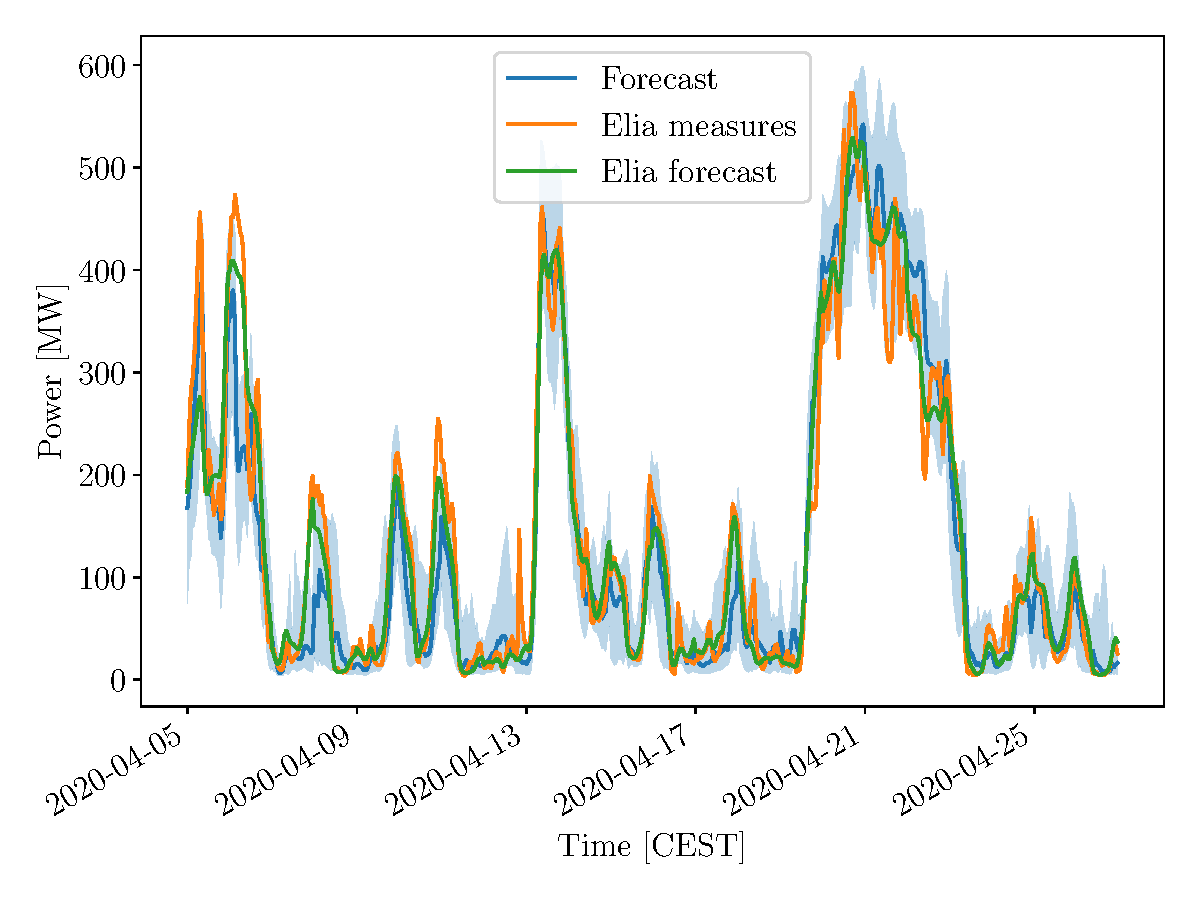
\includegraphics[width=.8\textwidth]{resources/pdf/wind_eval_qxt.pdf}
		\vspace{-1em}
		\caption{Quantile Extra Trees forecast}
		\label{fig:wind_eval_qxt}
	\end{figure}
	
	\begin{figure}
		\centering
		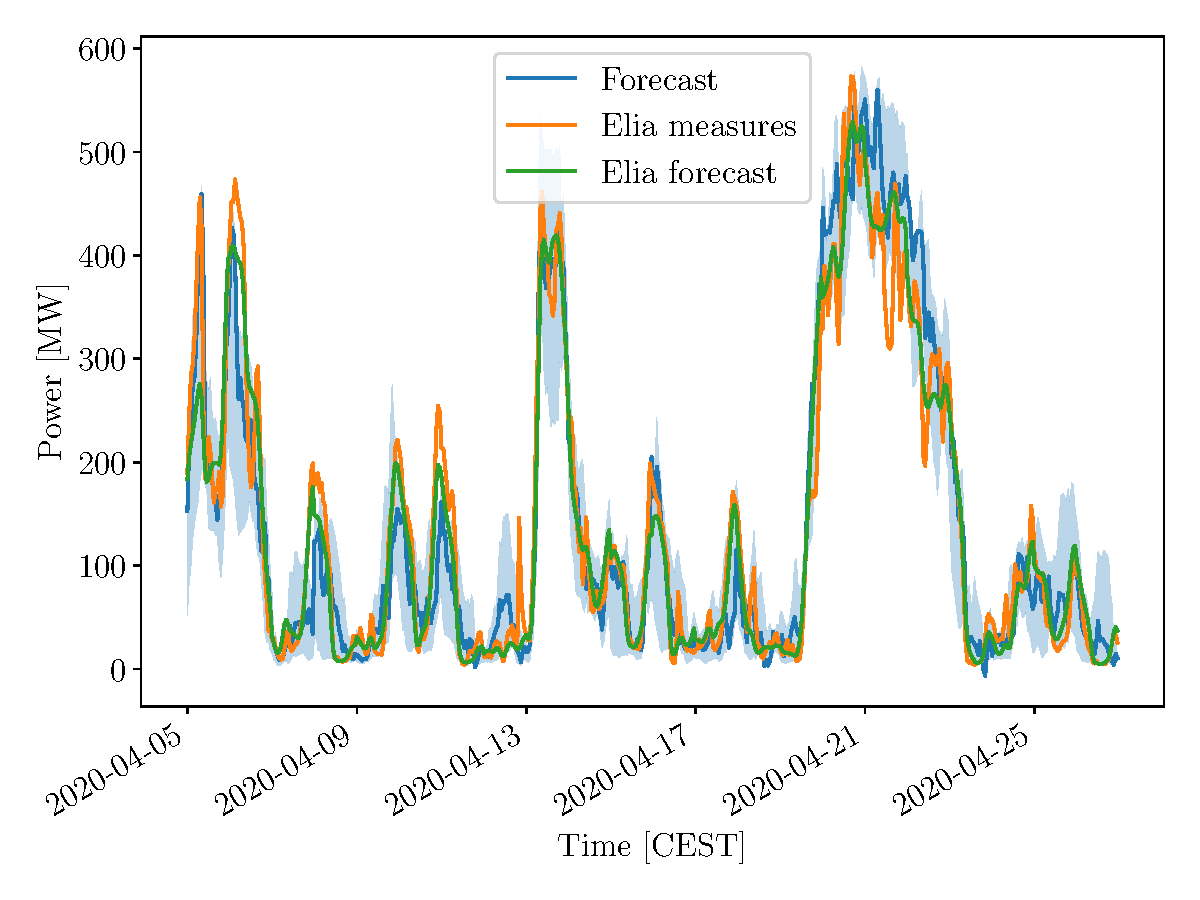
\includegraphics[width=.8\textwidth]{resources/pdf/wind_eval_qgb.pdf}
		\vspace{-1em}
		\caption{Quantile Gradient Boosting forecast}
		\label{fig:wind_eval_qgb}
	\end{figure}

	Moreover, on figures \ref{fig:wind_res_qxt} and \ref{fig:wind_res_qgb}, we can see the absolute residuals in order to get a more precise idea of the distribution of errors, and how they compare with Elia's errors.

	\begin{figure}[h]
		\centering
		\begin{subfigure}[t]{0.48\textwidth}
			\centering
			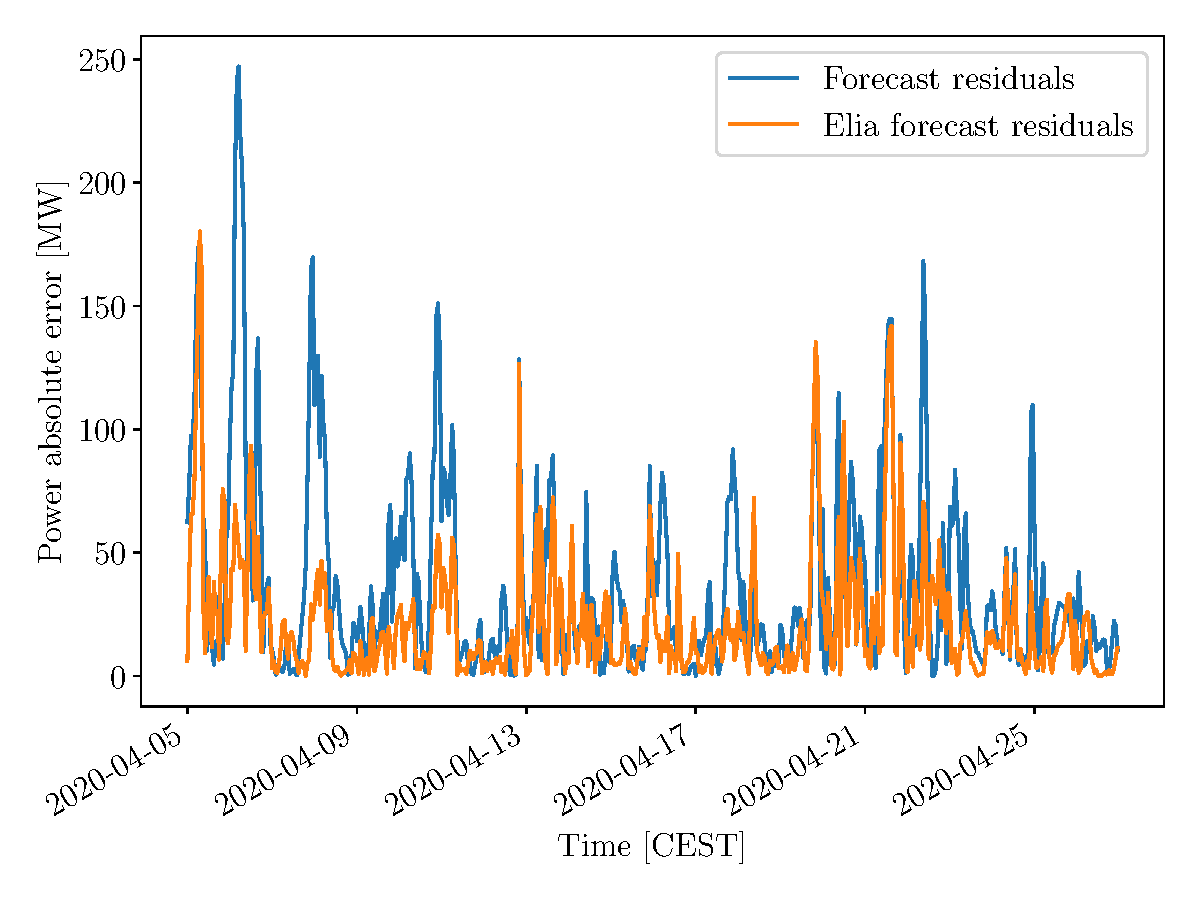
\includegraphics[width=\textwidth]{resources/pdf/wind_res_qxt.pdf}
			\caption{Quantile Extra Trees forecast residuals}
			\label{fig:wind_res_qxt}
		\end{subfigure}
		\hspace{0.5em}
		\begin{subfigure}[t]{0.48\textwidth}
			\centering
			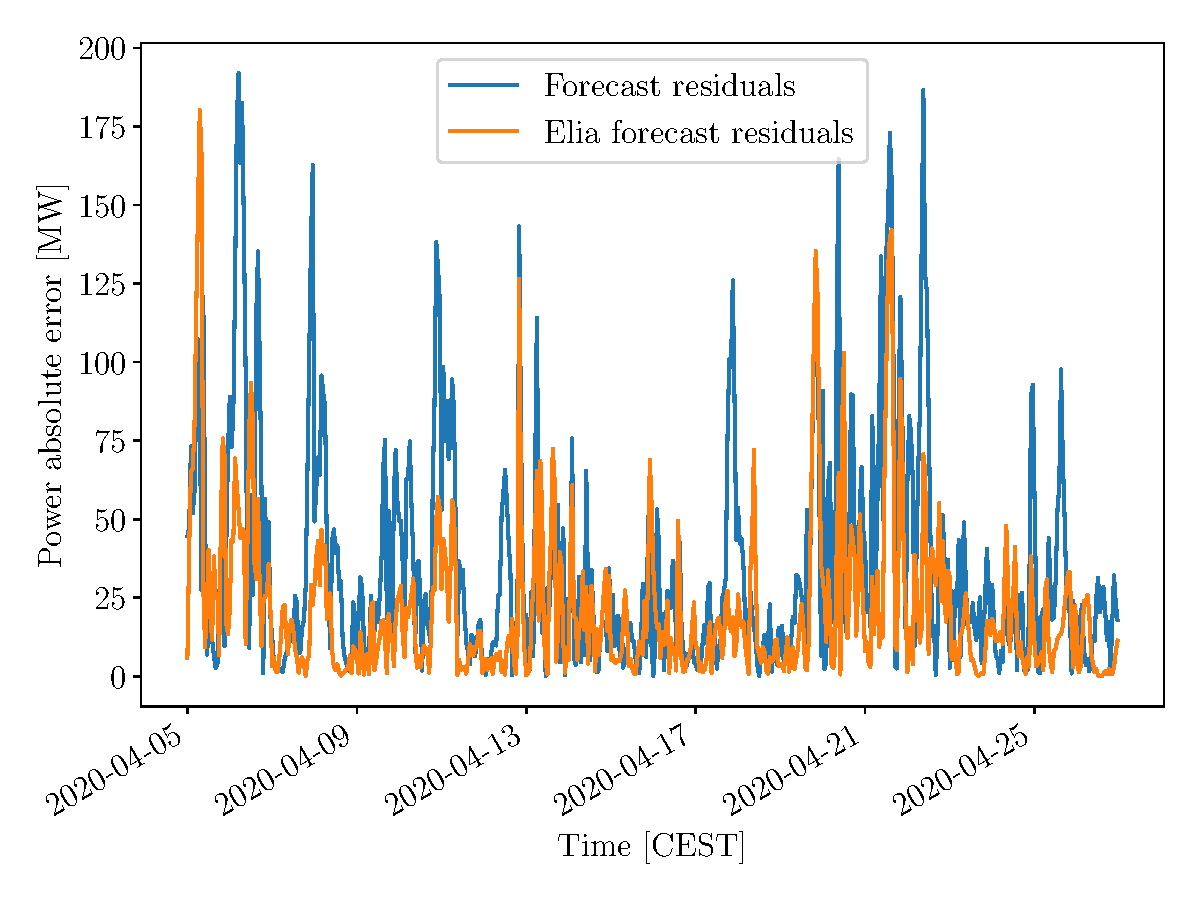
\includegraphics[width=\textwidth]{resources/pdf/wind_res_qgb.pdf}
			\caption{Quantile Gradient Boosting forecast residuals}
			\label{fig:wind_res_qgb}
		\end{subfigure}
		\caption{Residuals on \emph{weather forecast} test set}
	\end{figure}
	
	\subsubsection{Discussion}
	Let's go back to the numerical results of table \ref{tab:wind_test_set}.

	By comparing the first two test set, that have exactly the same size, we can notice, as was predicted earlier, that the strong correlation between the samples seems to have introduced a leakage of information from the learning set to the test set in the case of the shuffled TS. Then, we should not consider the results of the first test set as very reliable. Indeed, while the scores are comparable to those of Elia on the second test set, we are fraudulently better on the first test set.

	On the second test set, however, we have something that is quite encouraging, with a MAE around \SI{41}{\mega\watt} (corresponding to \SI{5.64}{\percent}) while Elia does \SI{40.16}{\mega\watt}. Obviously, if we reach results so close to Elia, it is because we work on weather measures instead of weather forecast like Elia that makes its prediction the day before.

	However, we have built a \emph{weather forecast} test set in order to assess how our model degrade when using in real condition: on weather forecast data. To compare things that are comparable, we have also used a \emph{weather measures} test set on the same period. This results are extremely good, with the MAE going from \SI{33.26}{\mega\watt} only to \SI{36.86}{\mega\watt} when going from weather measures to weather forecast for the Quantile Extra Trees, and from \SI{31.62}{\mega\watt} only to \SI{35.71}{\mega\watt} for the Quantile Gradient Boosting.

	Nevertheless, these results have to be nuanced. Indeed, on this very specific period our model has not degraded much at all. But this period is far from being exhaustive (only 22 days in April 2020), and we have a sign that this perior is not very representative of the general wind weather-power distribution. This can be inferred from the fact that while Elia has a MAE of only \SI{21}{\mega\watt} on this test set, while it has reached a MAE of \SI{34}{\mega\watt} on the shuffled test set, and \SI{40}{\mega\watt} on the last 6 months. That may be an sign that the considered period corresponds to a period were the forecasting was more “easy”.

	That being said, given the derivative of the sum of all wind power curves in Wallonia, we are confident that the MAE should less than double when used in forecasting mode, if we can count on day-ahead MAE of wind speed forecast below \SI{2.4}{\meter\per{\second}} \parencite{el-fouly2008wind}, even if we have no formal guarantee of that, as the power curve are not directly related to the learnt models.
	
	Nevertheless, the results are quite good, with a MAE on weather measurements very close than this of Elia (on weather forecast). Furthermore, we are quite happy with these results, as some of the best results at the regional level based on NWP are obtained by an hybrid approach called WPPT \parencite{croonenbroeck2014windpower}. In this paper, they showed that they reach results between \SI{3}{\percent} and \SI{15}{\percent} in terms of nRMSE depending on the case study, and here the results are between \SI{7}{\percent} and \SI{8}{\percent} on weather measurements.
		
	Finally, the two models are quite equivalents in term of performance, even if the Quantile Gradient Boosting seems to take the advantage for all the quantile losses (MQL). However, we think that it is preferable to use the Extra Trees for three reasons:
	\begin{itemize}
		\item They are really fast to train, we could thus profit from more data from Elia using a weather API that provide information every quarter, avoiding us the need to average the measures of Elia by four.
		\item They are slow to predict, but our task is to predict for the next day only, which is thus really fast.
		\item As a single tree is grown, and that quantiles for a given sample are estimated from the content of the same leaves, the quantiles are coherent. It means that a lower quantile is never above the upper quantile or the median prediction, while it can be the case with the three estimators built in the Quantile Gradient Boosting.
	\end{itemize}

\subsection{Limitations and possible improvements}

	To conclude on these results, we could say that they are very decent, although we have certainly not succeed in reaching the accuracy of Elia on the forecasting task (this could not be verified). In a word, we reach the results of Elia on forecast when using weather measures as input. The reason why Elia performs better could come from the fact that they have access to more precise data and weather measures, and maybe they have access to power data for each wind farm instead of aggregated data.
	
	Another limitation of our work is that the availability of data forced us to work at the Wallonia level, while the project was focused on Liege province. If we had to make predictions for the Liege province only, we would follow the following procedure:
	\begin{itemize}
		\item Forecasting the total wind power in Wallonia
		\item Forecasting the wind power at each power plant using the physical model (even if it clearly overestimates, each power plant receives a weight proportional to the cubed wind speed, in addition to respect the cut-in, cut-out and rated speeds)
		\item Multiplying the total wind power by the ratio of wind power coming the Liege province according to the physical model.
	\end{itemize}
	% And that is the best that we can do. Indeed, feeding the model with wind only for the province of Liege is a bad idea as it corresponds to an unseen situation. And taking the fraction of power in proportion to the feature importances at each power plant shouldn't work very well because of the multicolinearity between the inputs
	
	On the other hand, if we had to make predictions for the whole Wallonia, the solar power forecasting approach developed in the first two sections would be able to scale straightforwardly.
	
	Finally, an interesting follow up work on this part would be to go for a hybrid approach, where we post-process the output of the physical model (in addition to the weather data, or not). Indeed, as can be seen from figure \ref{fig:wind_phys}, the physical model, seems to be promising if we consider reshaping the power curves, for example by using a machine learning model between the physical model output and the corrected output.

\newpage
\part*{Conclusion}

A first general remark is that we find regrettable that a large part of the data we needed were either very hard or impossible to obtain. For instance, we looked for a long time after a training dataset for the panels mapping and we never found quality aerial images for the province of Liège. Also, finding free of access irradiance data took us quite some time, and we are still facing limitations: we can only request for one location, and will eventually be limited to 10 API calls a day. The same applies for the weather data retrieved for the wind power production part.

Another important remark concerning the data availability is that we weren't able to collect past forecast for the weather data, but only measures for the past. This is really annoying as it completely prevents us to provide performance metrics in real conditions for our models. We are limited to the few forecast data retrieved manually for the period of April 2020. 
Nevertheless, we are satisfied with the results obtained for each branch of this project.

Our photovoltaic panels mapping yields precise results, to a certain extent, and is sufficiently fast to cover large areas in a relatively low amount of time. Furthermore, as we implemented it, it could very well be applied to any region for which we have satellite images, with few additional overhead. However, we genuinely regret the lack of uncertainty about our estimations.

As far as our photovoltaic power models are concerned, we are quite surprised, hence satisfied, with the obtained accuracy in experimental settings (year 2019) but also in real-life settings (April). Also, even though Elia outperforms our models in a real-life setting, they still perform much better than simple baseline models. In addition, it should be kept in mind that Elia has very likely access to more and more accurate information than us and they could be using a much more complex model.

In regards to the wind power models, we are really satisfied with the results obtained in view of what we have seen as results in the scientific literature, and in view of the initial performance of our physical model. We may regret being (supposedly) outperformed by Elia on the forecast task. But, as mentioned above, this could be due to the differences in data sources between Elia and us. Future works could consider hybrid models, more complex or fine-tuned supervised learning models, and, if the data was available, learning smaller independent models for each wind farm.

Finally, in order to showcase our final results, we have built a little interactive website : \href{https://znkvzr.com/apps/big-data/}{\texttt{https://znkvzr.com/apps/big-data/}}. It should be updated with new forecasts daily.

The github repository including the photovoltaic panels mapping section can be found here: \href{https://github.com/francois-rozet/adopptrs/}{\texttt{francois-rozet/adopptrs}}.

The github repository including the photovoltaic power production and wind power production section can be found here: \href{https://github.com/lgaspard/repf/}{\texttt{lgaspard/repf}}.

\newpage

\printbibliography

\appendix

\section{Figures}

\begin{figure}
    \centering
    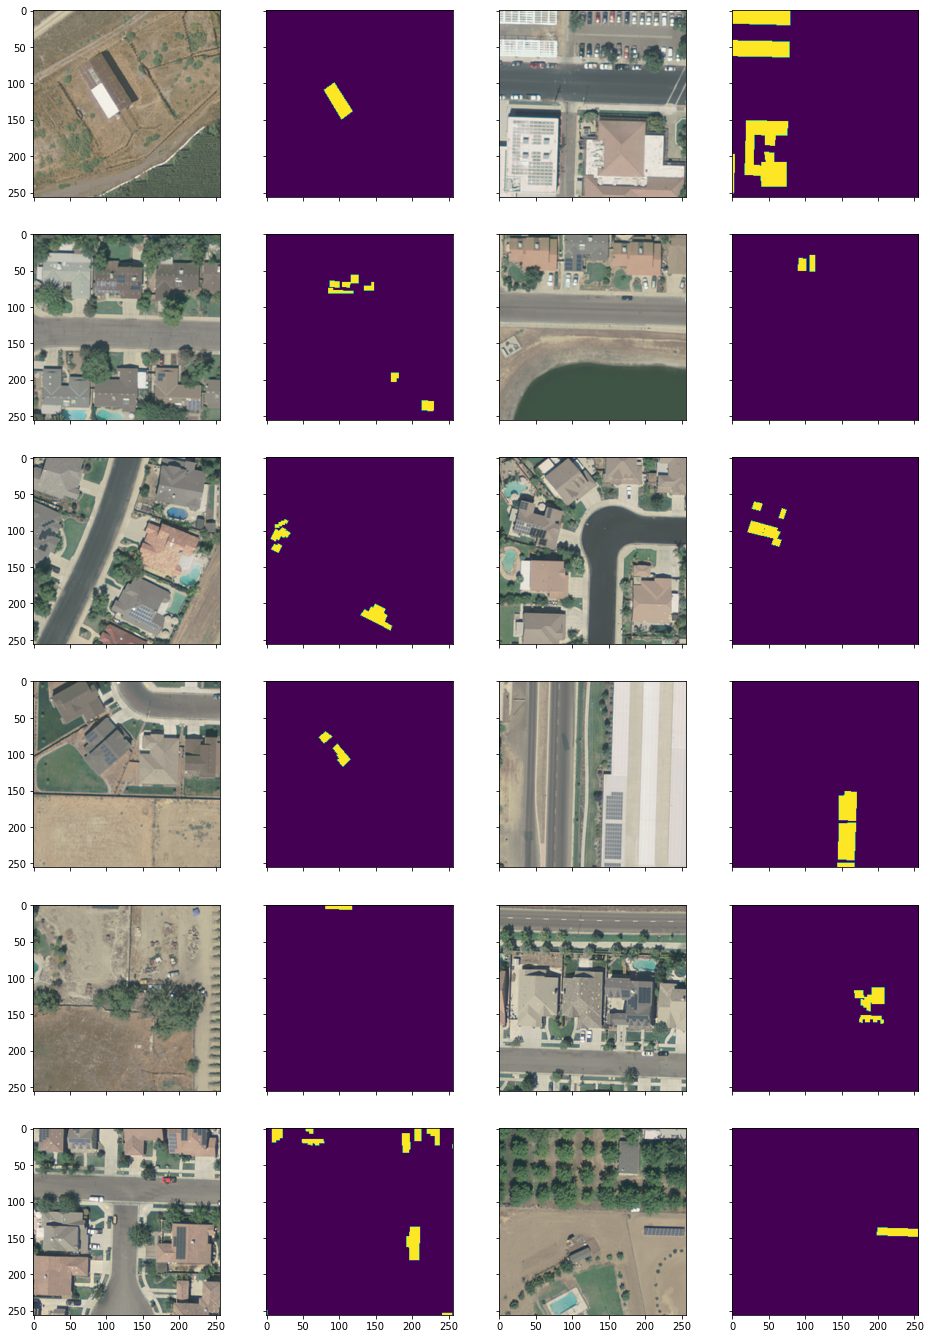
\includegraphics[width=\textwidth]{resources/png/masks.png}
    \noskipcaption{Californian dataset sample, with the produced masks.}
    \label{fig:masks}
\end{figure}

\begin{figure}
    \centering
    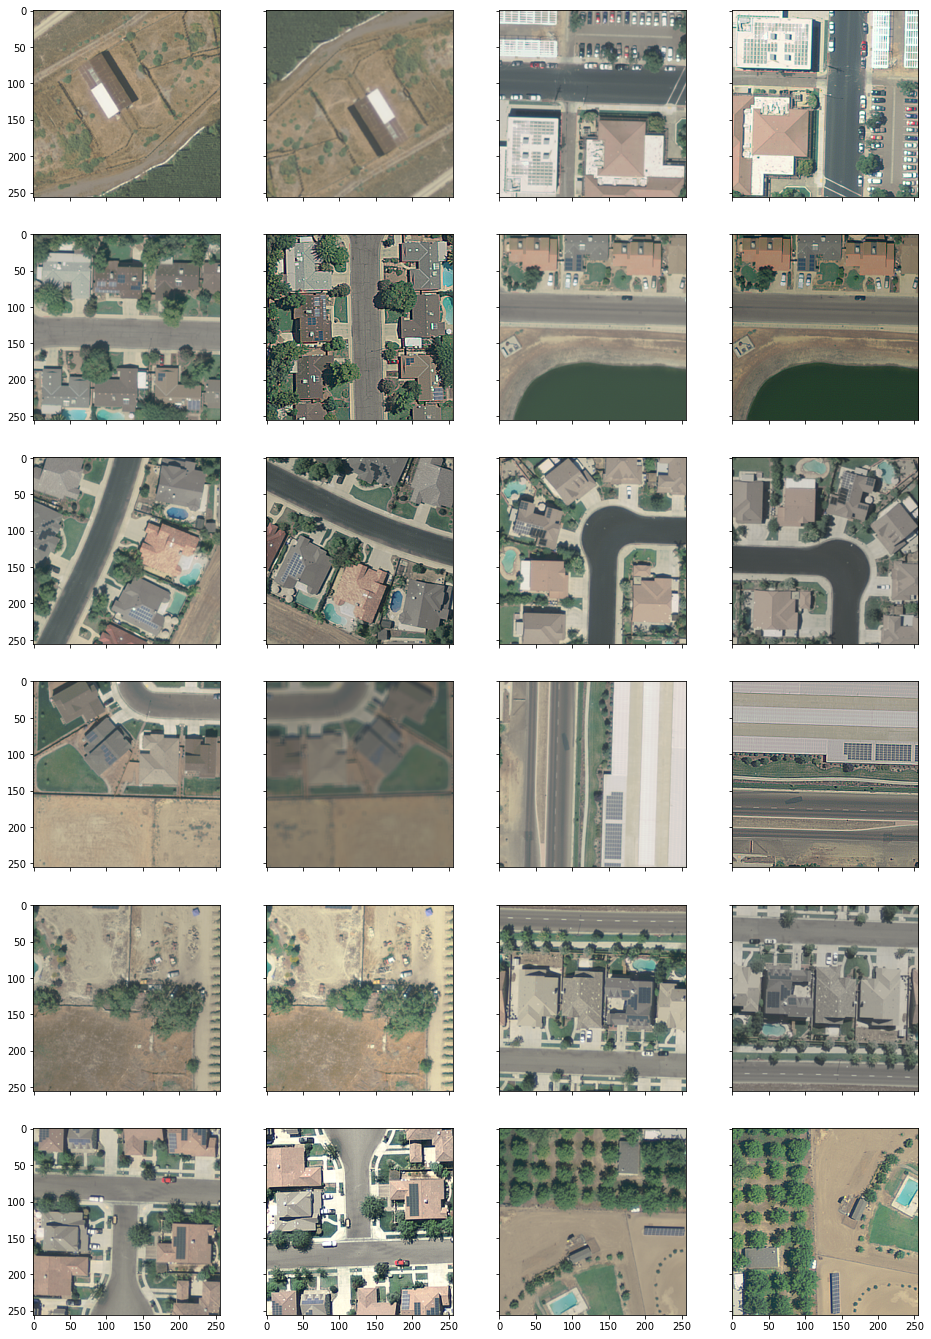
\includegraphics[width=\textwidth]{resources/png/augmentation.png}
    \noskipcaption{Californian original (left) vs augmented (right) dataset sample.}
    \label{fig:augmentation}
\end{figure}

\end{document}
